%%==================================================
%% chapter03.tex for SJTU Master Thesis
%% Encoding: UTF-8
%%==================================================

\chapter{Secure KVM:安全嵌套式虚拟化系统}
\label{chap:securekvm}



\section{引言}

随着云计算的不断发展,越来越多的云服务提供商以虚拟主机(Virtual Private Server)的形式为用户提供产品服务。对于用户而言,这种方式带来了无与伦比的灵活性,用户可以自定义虚拟主机上的操作系统、软件栈,就如同拥有一台真实的远程服务器一般。用户甚至可以给云服务提供商直接上传自己的虚拟机镜像,其应用程序便可以直接在云平台上运行,大大简化了部署的过程。对于云服务提供商而言,目前有丰富的开源虚拟化平台可供采用,通过将多台客户虚拟主机整合到单台物理机器上运行,其可以提高资源利用率,减少在硬件投入和能源消耗上的成本。总而言之,多租户云的普及,这是一个双赢的过程。

可是,事物总有其双面性,如何保障客户虚拟主机中敏感数据的安全性和私密性,是在多租户云环境中必须面对的一个突出问题。用户在虚拟主机中往往会保存一些敏感数据,如用于非对称加密的公私钥、存储用户名密码的数据库表等,由于现有虚拟化平台的局限性,这些敏感数据均能很容易地被恶意虚拟机监控器或者云服务提供商操作人员窥测到,存在泄漏的风险。

在本章中,我们借助嵌套式虚拟化,提出了一种透明、向前兼容的增强客户虚拟机中敏感数据安全的解决方案。通过在现有虚拟机监控器下方加入嵌套式虚拟化层,我们可以监控虚拟机监控器的行为,避免其对客户虚拟机的内存、磁盘数据安全造成威胁。Secure KVM以可接受的性能开销作为代价,保障了客户虚拟机中敏感数据的安全性与隐私性。

\section{背景介绍及问题分析}

\subsection{虚拟化本质论}

所谓“系统虚拟化”,亦即VMM虚拟机监控器给客户操作系统和应用程序提供一个虚拟的运行平台,而这个虚拟运行平台要与真实硬件基本无异,不能让客户操作系统和应用程序感受到差别(现阶段,打通VMM虚拟机监控器和Guest VM客户虚拟机之间的语义隔阂,主动让客户虚拟机意识到自己运行在虚拟化平台上以获得性能提升的情形也是存在的,在本文中我们忽略这样的特例)。

对于一个虚拟的运行平台而言,有三个主要组成要素,分别是CPU、内存和外设(磁盘和网卡属于此类)。关于CPU,虚拟机监控器要将物理机器上的计算资源即CPU时间片分一部分给客户虚拟机,同时又必须保证CPU资源不能被某一客户虚拟机长期无节制地占用,以免耽误虚拟机监控器自身和其他客户虚拟机的正常运行(类似于操作系统和应用程序之间的关系)。对于内存,虚拟机监控器同样要在满足客户虚拟机内存资源分配的同时保证安全,即某一客户虚拟机必须有节制地使用内存,该客户虚拟机和虚拟机监控器、该客户虚拟机和其他客户虚拟机之间必须保证内存隔离。对于外设,虚拟机监控器要对他们的IO行为进行精确模拟,这一般是通过截获IO指令和MMIO读写操作来完成。

这所有的一些,均要求虚拟机监控器处在比客户虚拟机更高的运行级别。对于CPU,虚拟机监控器要在某一客户虚拟机时间片用完时(时间中断到来),立即获得执行机会抢占该客户虚拟机,并切换另一客户虚拟机上来运行。对于内存,虚拟机监控器要通过一些类似页表的硬件机制限制客户虚拟机的访存范围。对于截获IO指令和MMIO读写,这同样需要高运行级别和硬件机制来保证。

具体到x86硬件虚拟化,虚拟机监控器处在高权限级别的根模式(root mode),客户虚拟机处在低权限级别的非根模式(non-root mode)。当客户虚拟机处在非根模式运行期间发生时间中断时,处理器会以外部中断(External Interrupt)到来的原因陷入到根模式,让虚拟机监控器处理。2007之后Intel推出的第二代硬件虚拟化处理器,均支持扩展页表(Extended Page Table,简称EPT),可以在硬件层面上限制客户虚拟机的内存访问。最后,虚拟机监控器可以指定IO位图,让非根模式下期望的IO指令发生陷入(MMIO读写与此基本类似),并对其进行指令模拟以达到模拟真实设备行为的目的。

不可否认,为了达到系统虚拟化的目的,在一般情况下让虚拟机监控器处在高权限级别是一个必要条件。但与此同时带来的是,虚拟机监控器不受管控的“为所欲为”,给客户虚拟机运行的安全性和隐私性带来了重大隐患。此情形在多租户云、第三方虚拟机提供商等应用环境下体现得尤为明显。下面两节分别从内存和磁盘的角度对此进行详细阐述。

\subsection{客户虚拟机的内存安全}

客户虚拟机的内存中包含有其正在运行程序的所有信息,包括操作系统层面的进程信息、模块信息和应用程序地址空间中的所有数据、代码区域。举例来说,客户虚拟机中的浏览器打开了网银的登录界面而用户正在输入其账号密码,这些隐私数据都是会被保存到客户虚拟机的内存中。

扩展页表限制的是客户虚拟机的访存范围,而虚拟机监控器处在最高权限级别,其可以将物理上的任意内存区块映射到自己的地址空间,并进行访问改写。同样以上文用户网银登陆为例,恶意虚拟机监控器在得知这一信息后,可以对整个客户虚拟机的内存空间进行转储(dump),并在事后进行查找分析,导致用户的敏感隐私数据极有可能因此而被暴露偷窥。

尽管恶意虚拟机监控器起先获取的可能只是庞杂的原始字节数据,其可以利用特殊寄存器数据、特定操作系统内存地址空间结构等信息作为提示,借助虚拟机自省(Virtual Machine Introspection,VMI)等技术手段,从中萃取出隐私数据和语义信息,毕竟这在理论上是可能的。

\subsection{客户虚拟机的磁盘安全}

在真实机器上读磁盘的过程可以简化为此,操作系统先在内存中预留一段区域,然后将待读取数据在磁盘上的位置和预留内存地址等信息通过IO指令告诉磁盘,磁盘通过直接内存访问(Direct Memory Access,DMA)将数据填写到预留内存区域,最后发送中断告诉操作系统数据已经准备就绪。写磁盘的过程基本与此类似。在虚拟化环境下,虚拟机监控器模拟了上述DMA的过程,其在根模式截获敏感IO指令,从磁盘映像中获取对应数据并填至客户虚拟机内存,最后注入虚拟中断告知完成。可以看到,虚拟机监控器处在客户虚拟机的IO数据路径之中,其可以对磁盘IO数据进行任意偷窥甚至修改,威胁客户虚拟机的磁盘安全。

此外,客户虚拟机的磁盘映像直接以明文形式保存在虚拟机监控器中,恶意虚拟机监控器可以在挂载该磁盘映像后对其中文件系统进行任意查看和改动,以更直接的方式对客户虚拟机的磁盘安全造成威胁。



\section{Secure KVM系统的设计}

\subsection{嵌套式虚拟化}

如果虚拟机监控器仍处于系统中的最高权限运行级别,那么能对其进行行为监控的只有处于
更低级别的处理器硬件了,这在目前的角度来看显然是不实际的。因此为了达到目的,我们
只能降低原虚拟机监控器的运行级别(即将其从根模式移出至非根模式),而让我们用于监
控虚拟机监控器行为的可信代码在最高权限级别根模式运行。这样,有了处理器硬件上不同
权限级别的保证,原虚拟机监控器中所进行的一切敏感操作都能被可信监控代码截获并进行
检查,从而保证客户虚拟机的运行安全,此即为安全嵌套虚拟化的主要思想。

\begin{figure}[!htp]
  \centering
  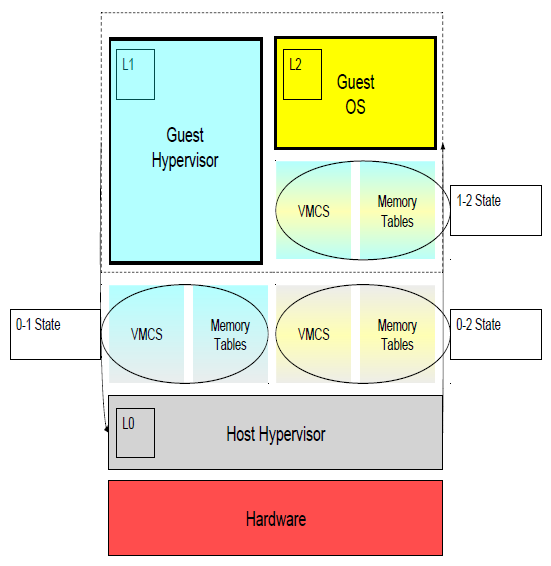
\includegraphics[width=0.7\textwidth]{chap3/nested.png}
  \bicaption[fig:nested]{嵌套式虚拟化示意}{嵌套式虚拟化示意}{Fig}{Illustration on Nested Virtualization}
\end{figure}

图\ref{fig:nested}展示了典型嵌套式虚拟化平台的主体结构,其中主要包含了L0、L1和L2三个层次。

\begin{itemize}
\item{L0(Host hypervisor):嵌套式虚拟化层,处于根模式运行。L1和L2中发生VMExit后均会陷入至此。}
\item{L1(Guest hypervisor):即为原虚拟机监控器,处于非根模式运行。为L2提供运行虚拟化支撑的同时受到L0的管控。}
\item{L2(Guest VM):即为原客户虚拟机,处于非根模式运行。用户应用程序在此运行。}
\end{itemize}

x86处理器硬件上主要有两个结构对非根模式下的运行进行控制,分别是VMCS(Virtual Machine Control Structure)和EPT。嵌套式虚拟化层L0为了支撑原虚拟机监控器L1的运行,为其准备了VMCS和EPT,我们将这一部分状态定义为“0-1状态”。原虚拟机监控器L1为了支撑原客户虚拟机L2的运行,同样为其准备了VMCS和EPT,我们将这一部分状态定义为“1-2状态”。然而,x86处理器没有从硬件上直接支持多层嵌套虚拟化(只有根模式和非根模式两种运行权限级别),也就是说实际上L1和L2处在同样的权限级别均在L0的管控下直接运行,因此L0需要为L2的运行提供额外的VMCS和EPT(相当于0-1状态和1-2状态的合并),我们将其定义为“0-2状态”。下文说明了嵌套式虚拟化系统运行的一个典型流程。

\begin{enumerate}
\item L0以VMCS0-1运行L1
\item L1准备VMCS1-2并执行vmlaunch/vmresume启动L2
\item vmlaunch产生陷入至L0,执行流由L0接管
\item L0将VMCS0-1和VMCS1-2合并,生成VMCS0-2
\item L0以VMCS0-2运行L2
\item L2在非根模式下运行,一段时间后产生陷入
\item 执行流再次由L0接管,L0根据VMExit类型选择自己处理或传递给L1处理
\item 如果L0自己能处理陷入,则vmresume继续执行L2。如果必须交给L1处理,L0根据VMCS0-2准备VMCS0-1和VMCS1-2,并将执行流切换到L1
\item 在1$\sim$8或5$\sim$8之间重复
\end{enumerate}

\subsection{系统整体架构}

\begin{figure}[!htp]
  \centering
  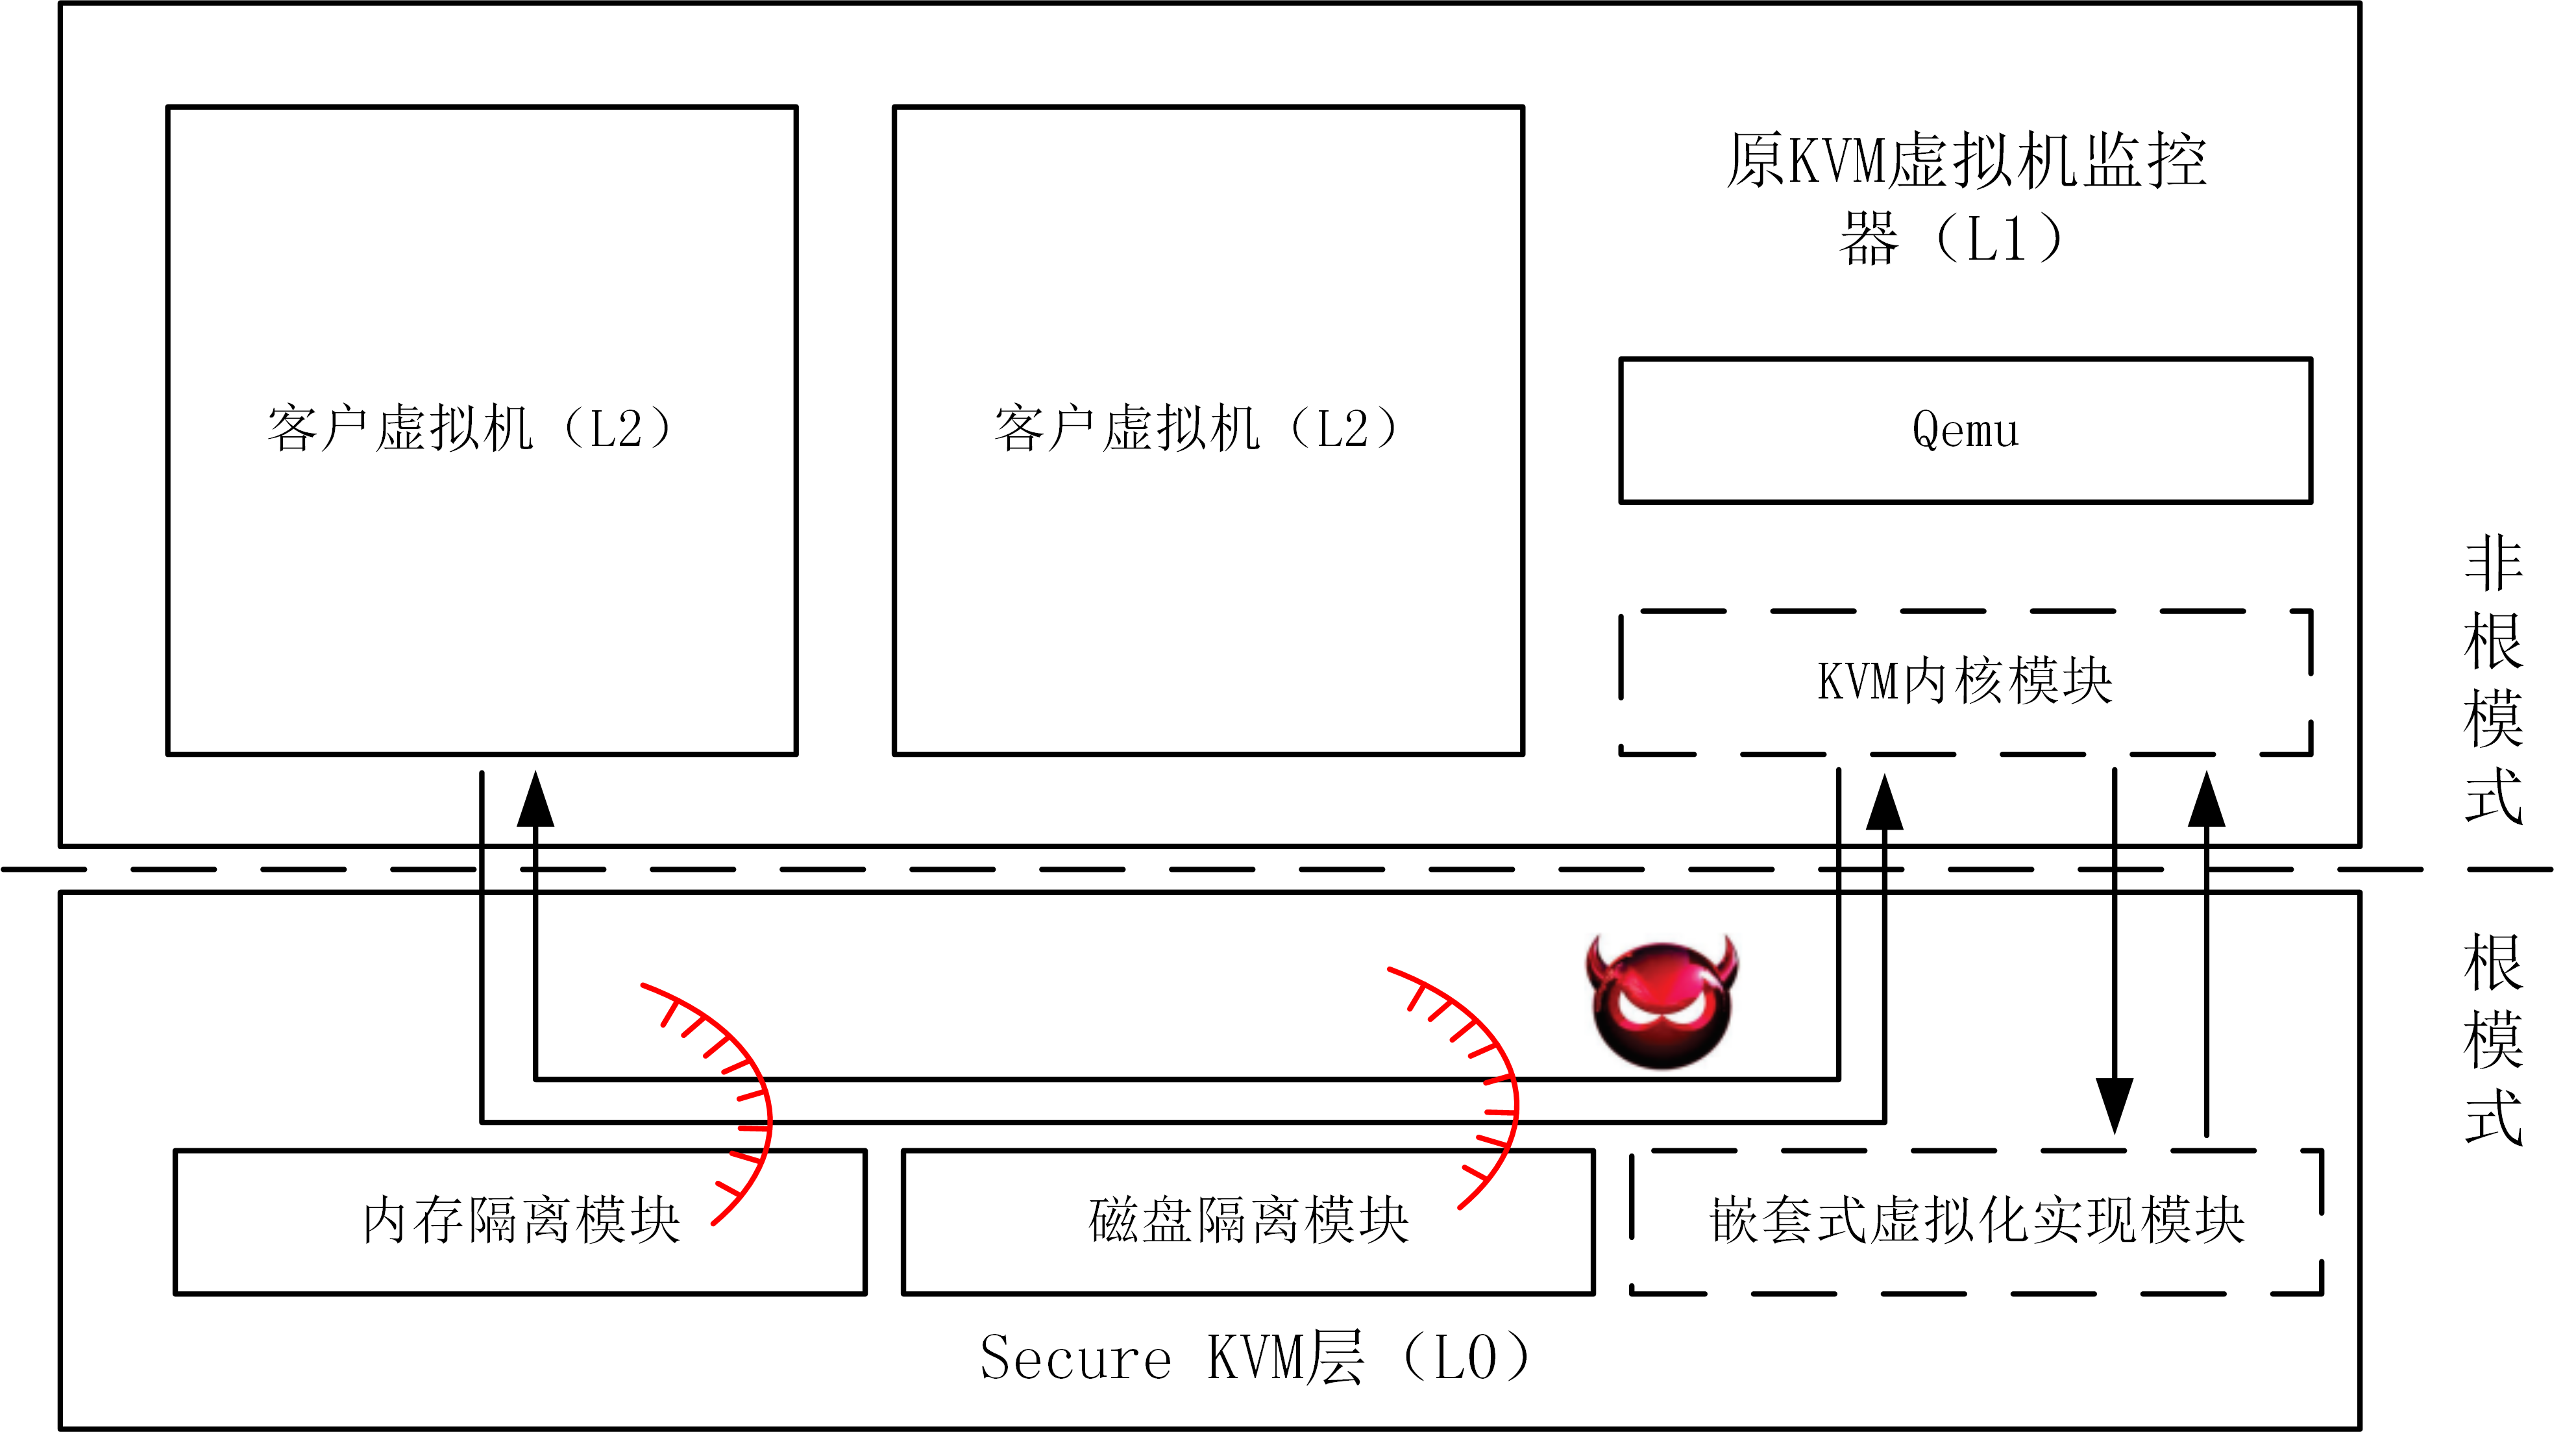
\includegraphics[width=0.9\textwidth]{chap3/architecture.png}
  \bicaption[fig:architecture]{Secure KVM系统整体架构示意}{Secure KVM系统整体架构示意}{Fig}{Illustration on System Architecture of Secure KVM}
\end{figure}

Secure KVM系统的整体架构如图\ref{fig:architecture}所示。Secure KVM在原KVM虚拟机监控器(L1)下方添加了安全嵌套式虚拟化层(L0)以占据系统最高权限,并将原先在VMX根模式下运行的KVM降权至非根模式运行。经过此番调整,L0便能对L1中针对L2客户虚拟机进行的任何敏感操作进行监视,放行正常的运行支持操作譬如I/O设备模拟,同时阻止非法的攻击行为如映射L2的无关内存页。这是因为在非根模式下执行敏感指令(如VMX指令)均会产生到L0的陷入,L0有机会对L1正在进行的操作进行检查确认,另外尤为重要的一点是,L0能够利用EPT硬件机制限制L1虚拟机监控器的访存范围。

Secure KVM于安全嵌套式虚拟化层内置了内存隔离模块和磁盘隔离模块,分别用于保障客户虚拟机的内存数据安全和磁盘数据安全。内存隔离模块的主要职责在于根据L1、L2实际运行情况灵活维护动态白名单和EPT表,维持L2正常运行的同时不让L1接触无关内存页。磁盘隔离模块的主要职责在于适时地对L2磁盘操作数据进行加解密,保证L1始终接触到的只能是密文数据。以上两模块在功能实现中存在小部分重叠,因为L2磁盘操作中有涉及L1对L2缓冲区的内存访问。

以上两模块的具体设计与实现将在接下来的两节中进行详细阐述。

\section{对客户虚拟机内存数据的安全保护}

\subsection{基本原理}

\begin{figure}[!htp]
  \centering
  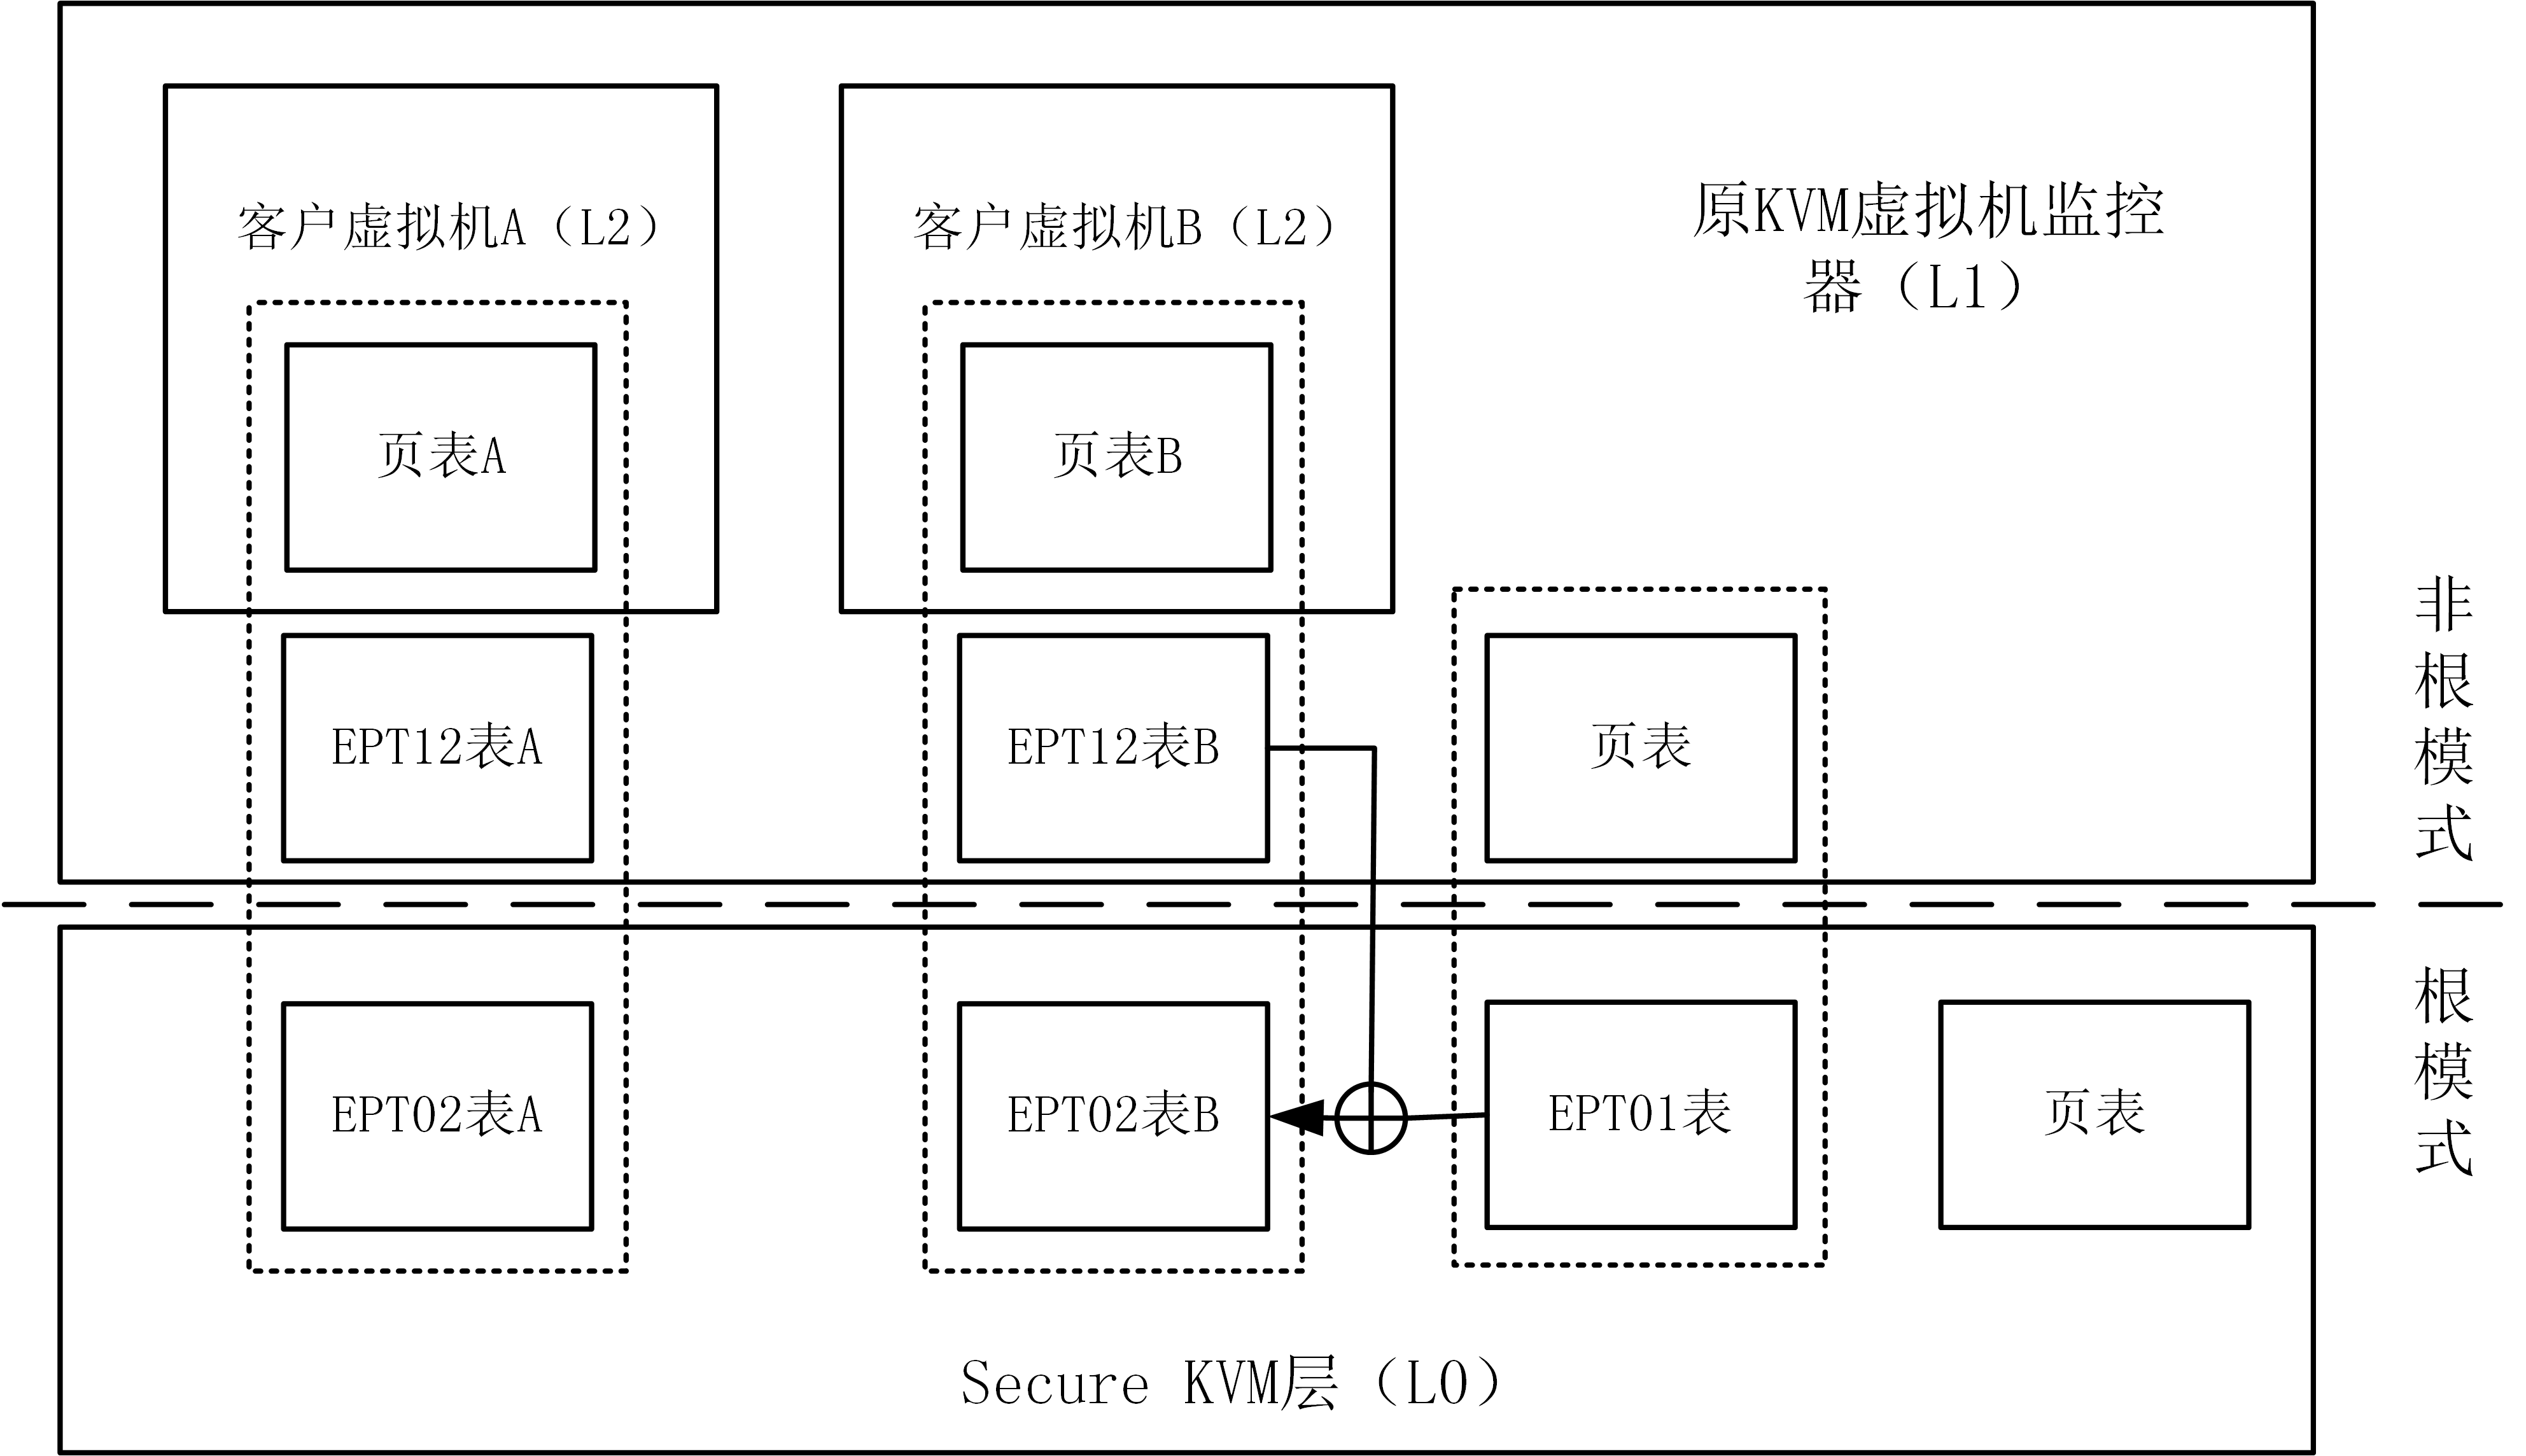
\includegraphics[width=0.9\textwidth]{chap3/mem_protect.png}
  \bicaption[fig:mem_protect]{Secure KVM系统中的内存管理机制示意}{Secure KVM系统中的内存管理机制示意}{Fig}{Illustration on Memory Management in Secure KVM}
\end{figure}

图\ref{fig:mem_protect}表示了Secure KVM系统中的内存管理机制。在嵌套式虚拟化环境中,L1和L2的内存访问是在处理器硬件的辅助下通过两张页表来完成的,其内存地址的翻译要经历从GVA(Guest Virtual Address)到GPA(Guest Physical Address)、和从GPA到HPA(Host Physical Address)的两层转换过程。处理从GVA到GPA翻译的页表位于L1和L2内部,由L1和L2自身负责维护,其实就是x86体系结构中处理虚拟线性地址到物理地址转换的页表(Page Table,PT)。处理从GPA到HPA翻译的页表位于L0嵌套式虚拟化层内,由L0负责维护,其实就是Intel在第二代硬件虚拟化扩展中提出的辅助扩展页表(Extended Page Table,EPT)。在Secure KVM系统中,我们将负责处理L1中GPA到HPA翻译的EPT称为EPT01表,将负责处理L2中GPA到HPA翻译的EPT称为EPT02表。事实上,在L1原虚拟机监控器内部,为了支持L2客户虚拟机的运行,还为其维护了一张EPT表,负责处理L2 GPA到L1 GPA的转换,而EPT02表实际是EPT01表和这张表的整合,我们将其称为EPT12表。在L2客户虚拟机运行时,EPT12表没有被加载入处理器硬件。

Secure KVM系统的一个设计目的是保护L2客户虚拟机内存数据的安全性,即在L1虚拟机监控器和L2之间建立内存隔离,禁止L1随意访问和修改L2的内存,从而避免L2内存空间中的敏感数据向L1泄露。

由图\ref{fig:mem_protect}可得知,L1的内存访问范围受到EPT01表的控制。因此,L0只需要将属于L2的内存区域从EPT01表中去除即可达到目的,这便是内存数据安全保护的大体原理。但是如果仅仅做到这一点,L2客户虚拟机便不能再正常启动,这是因为L1虚拟机监控器为了支持L2客户虚拟机正常运行为其提供了诸如IO外设模拟、指令模拟等多种基础服务。而这些基础服务不可避免地要去访问原本属于L2的内存空间,例如L1在为L2模拟磁盘读取时需要将被读取数据从磁盘映像拷贝至L2内存缓冲区,又如L1在模拟L2的in指令或MMIO读取时需要将数据写入某个属于L2的特定内存地址。

在Secure KVM系统中,我们借助于建立临时白名单来应对可能出现的例外情况。如果L1出于某种正当理由要对属于L2的内存区域进行访问,L2客户虚拟机之前必定会凭借虚拟化陷入让L0获知其即将进行的会产生例外的行为,如L2进行磁盘读取时涉及到的IO指令会产生到L0的陷入,又如进行MMIO读取时尽管使用的是普通mov指令,其仍然会产生到L0的陷入。L0在获知L2即将进行的行为后,根据相应规则,将L1在模拟该行为过程中可能访问到的L2内存区域加入临时白名单,并在EPT01表中添加这部分内存区域。如此一来,L1接下来便能正常地对L2所要求之行为进行模拟。等到L1对特殊行为完成模拟后,L0便会将这部分内存区域从临时白名单中去除,再次对EPT01表进行删改。这样,L0在维持L2客户虚拟机正常运行的同时,保护了其内存数据的安全。

\subsection{磁盘读写部分的特殊处理}

L2客户虚拟机在运行时不可避免要涉及到磁盘操作,而磁盘操作是由L1原虚拟机监控器为之模拟的。磁盘操作可被分为磁盘读取和磁盘写入,L1在模拟磁盘读取时需要往L2内存空间写入被读取的磁盘数据,在模拟磁盘写入时需要从L2内存地址空间读取待写入的磁盘数据。下文将分成PIO读、DMA读和DMA写三部分来具体讨论。

PIO读在初始阶段会往地址为0x1F2$\sim$0x1F5的IO端口写入待读取磁盘扇区信息,随后会用一条带REP指令前缀的INS指令来接收数据,存放数据的缓冲区内存地址由ES:EDI给出。L0在截获这条REP INS指令后,根据ES:EDI计算出被指定为缓冲区的L2内存地址,将涉及到的内存页面加入临时白名单,再将执行流交予L1。L1在接下来正常执行中会模拟REP INS指令在真实硬件上的行为,将对应的磁盘数据填充至内存缓冲区,在此过程中发生的缺页故障请求,由于对应的内存页面信息在白名单中已做记录,均会获得L0批准。待到L1完成模拟这次PIO读请求后,执行流会重新回到L0,L0再将这部分内存页面从EPT01表和白名单中清除,L1以后便不能再访问这部分内存。以上过程用顺序图表示如下。

\begin{figure}[!htbp]
  \centering
  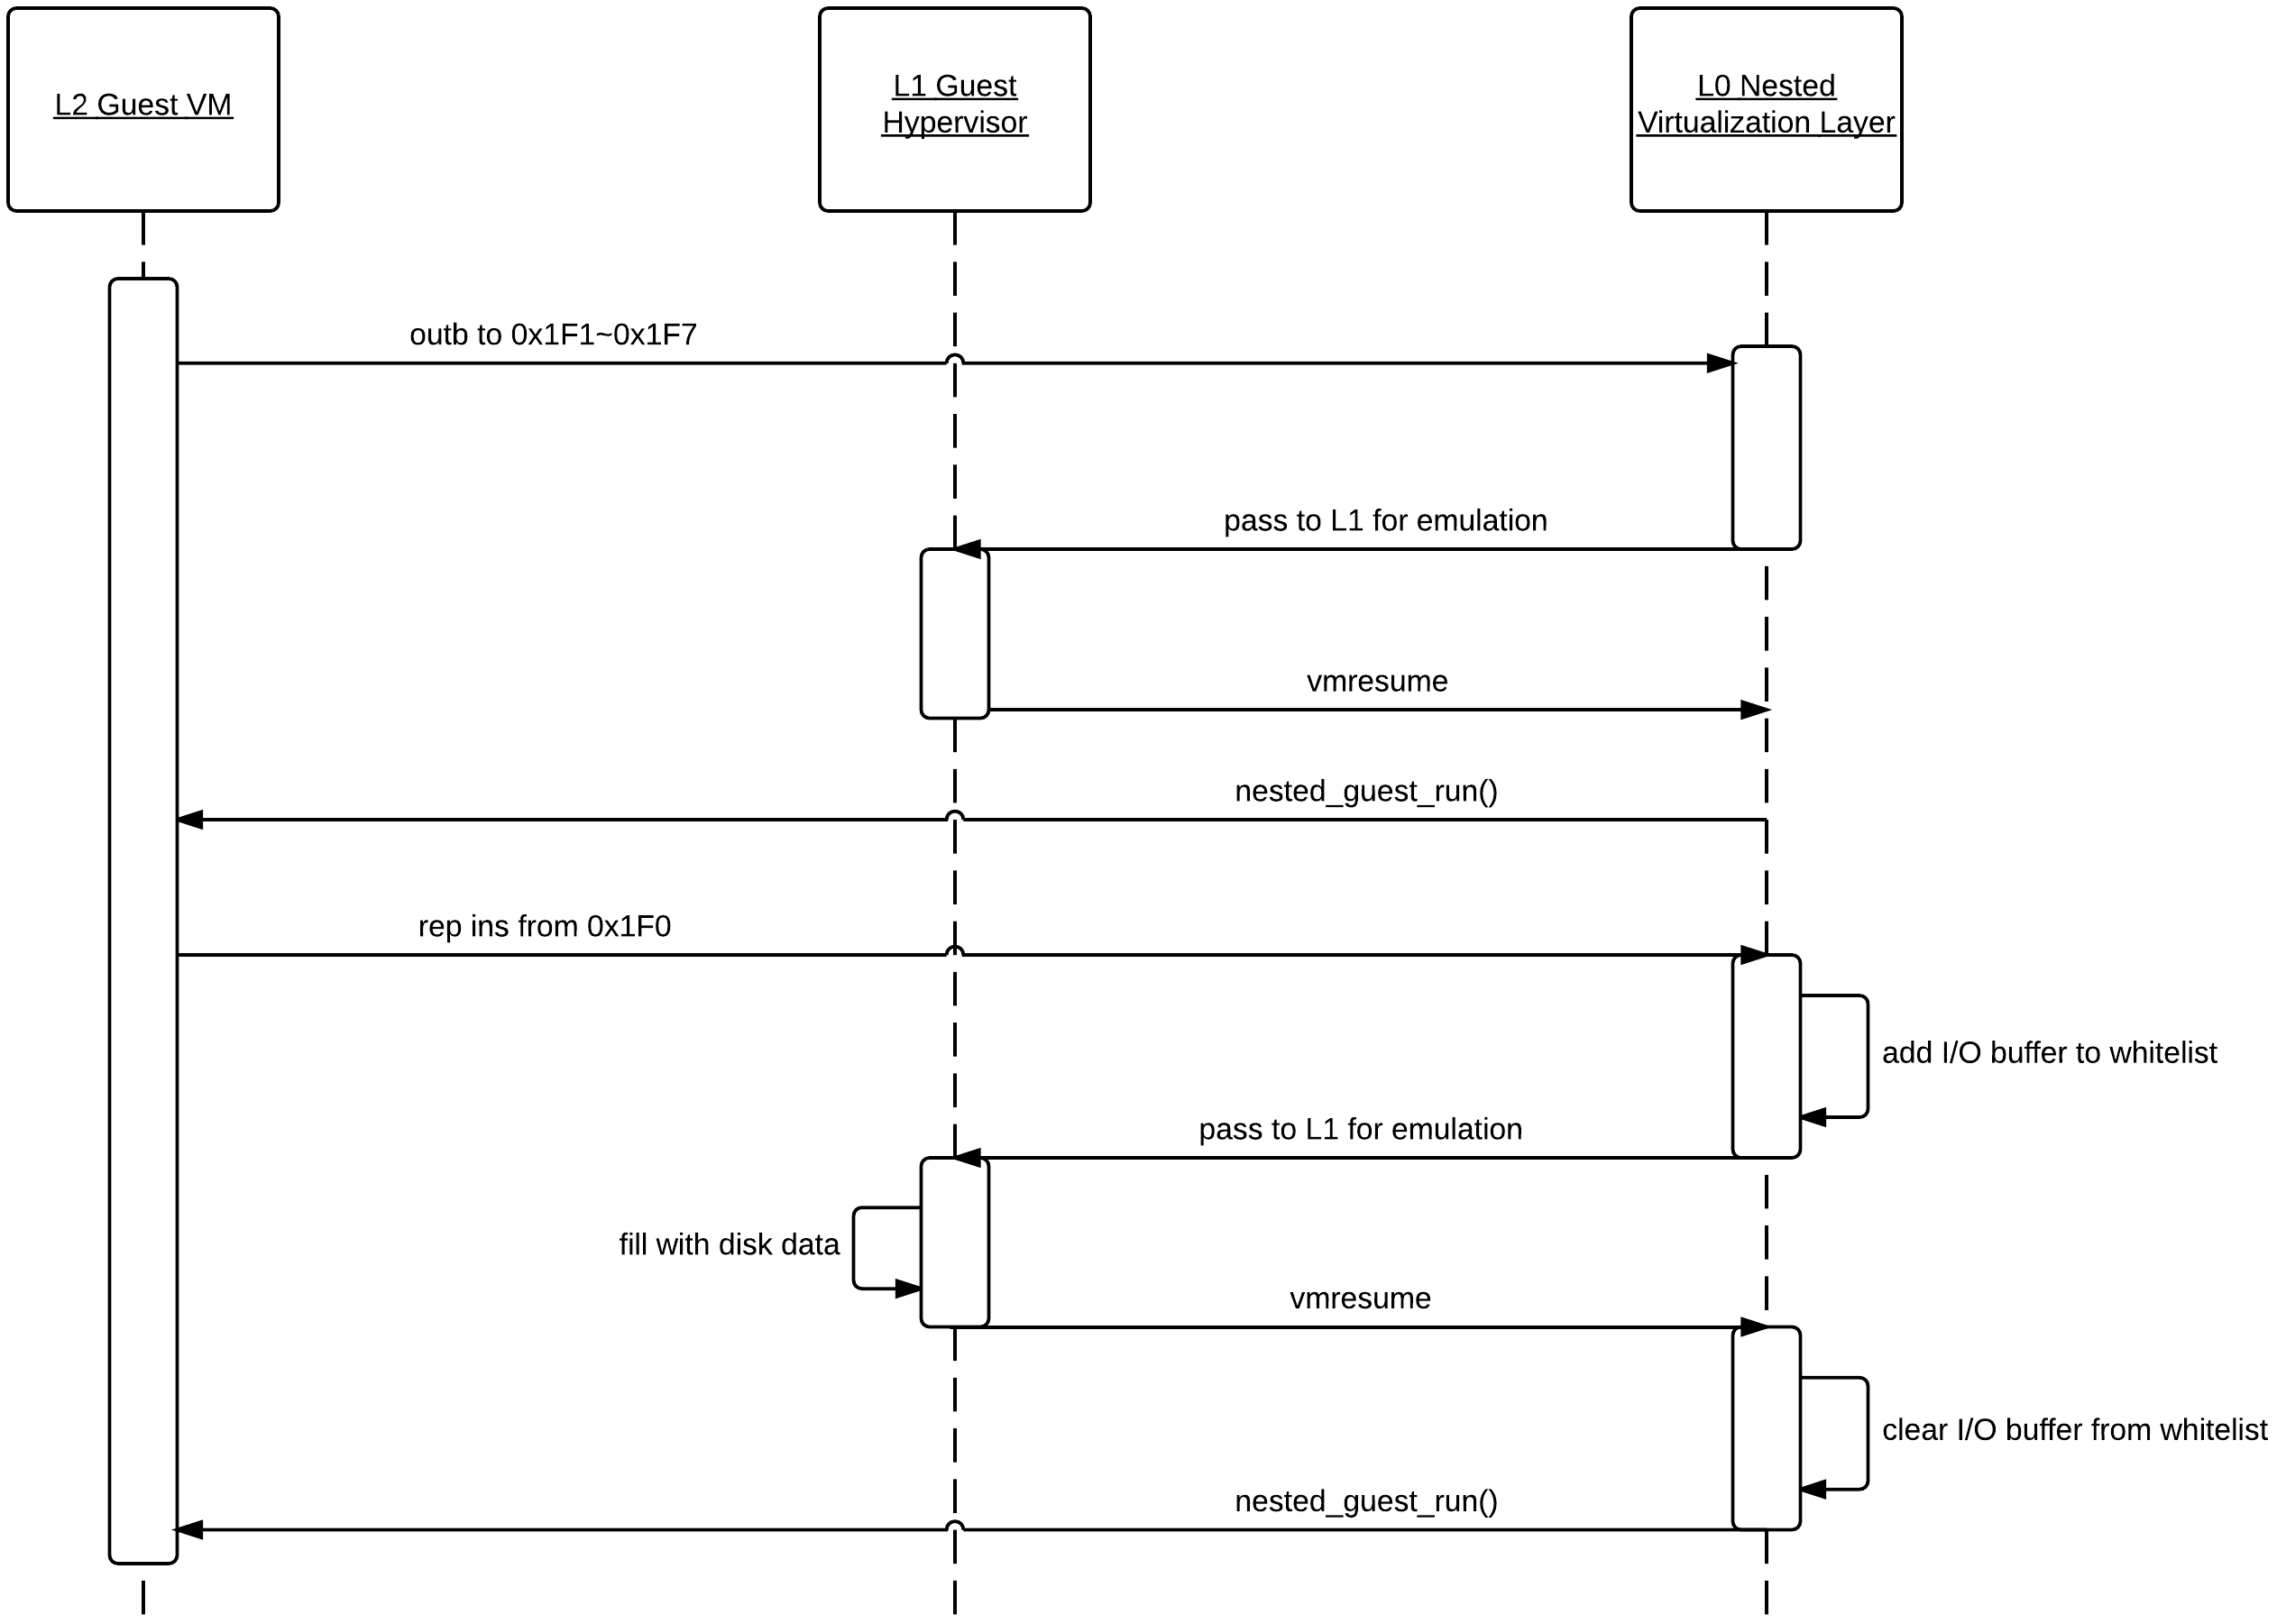
\includegraphics[width=0.95\textwidth]{chap3/pio_read2.png}
  \bicaption[fig:pio_read2]{PIO读取之内存保护顺序图}{PIO读取之内存保护顺序图}{Fig}{Sequence Diagram of memory protection on PIO Read}
\end{figure}

DMA读涉及到的流程和PIO读有些许不同,这是一个异步过程。DMA读在初始阶段也会往地址为0x1F3$\sim$0x1F5的IO端口写入待读取磁盘扇区信息,然后往0xC224端口写入PRDT表地址信息,最后往0xC220端口发出DMA读开始指令。PRDT表中以类似于集散序列的结构记录了
被用作缓冲区的内存区块信息,L0从中可以萃取出白名单信息,并在DMA读过程中对正常的缺页故障请求予以放行。L1在完成DMA读模拟后,会往L2注入虚拟设备中断,此时执行流会重新回到L0,L0以此为这次DMA读结束的界限,会对EPT01表和白名单进行清理。以上过程用顺序图表示如下。

\begin{figure}[!htbp]
  \centering
  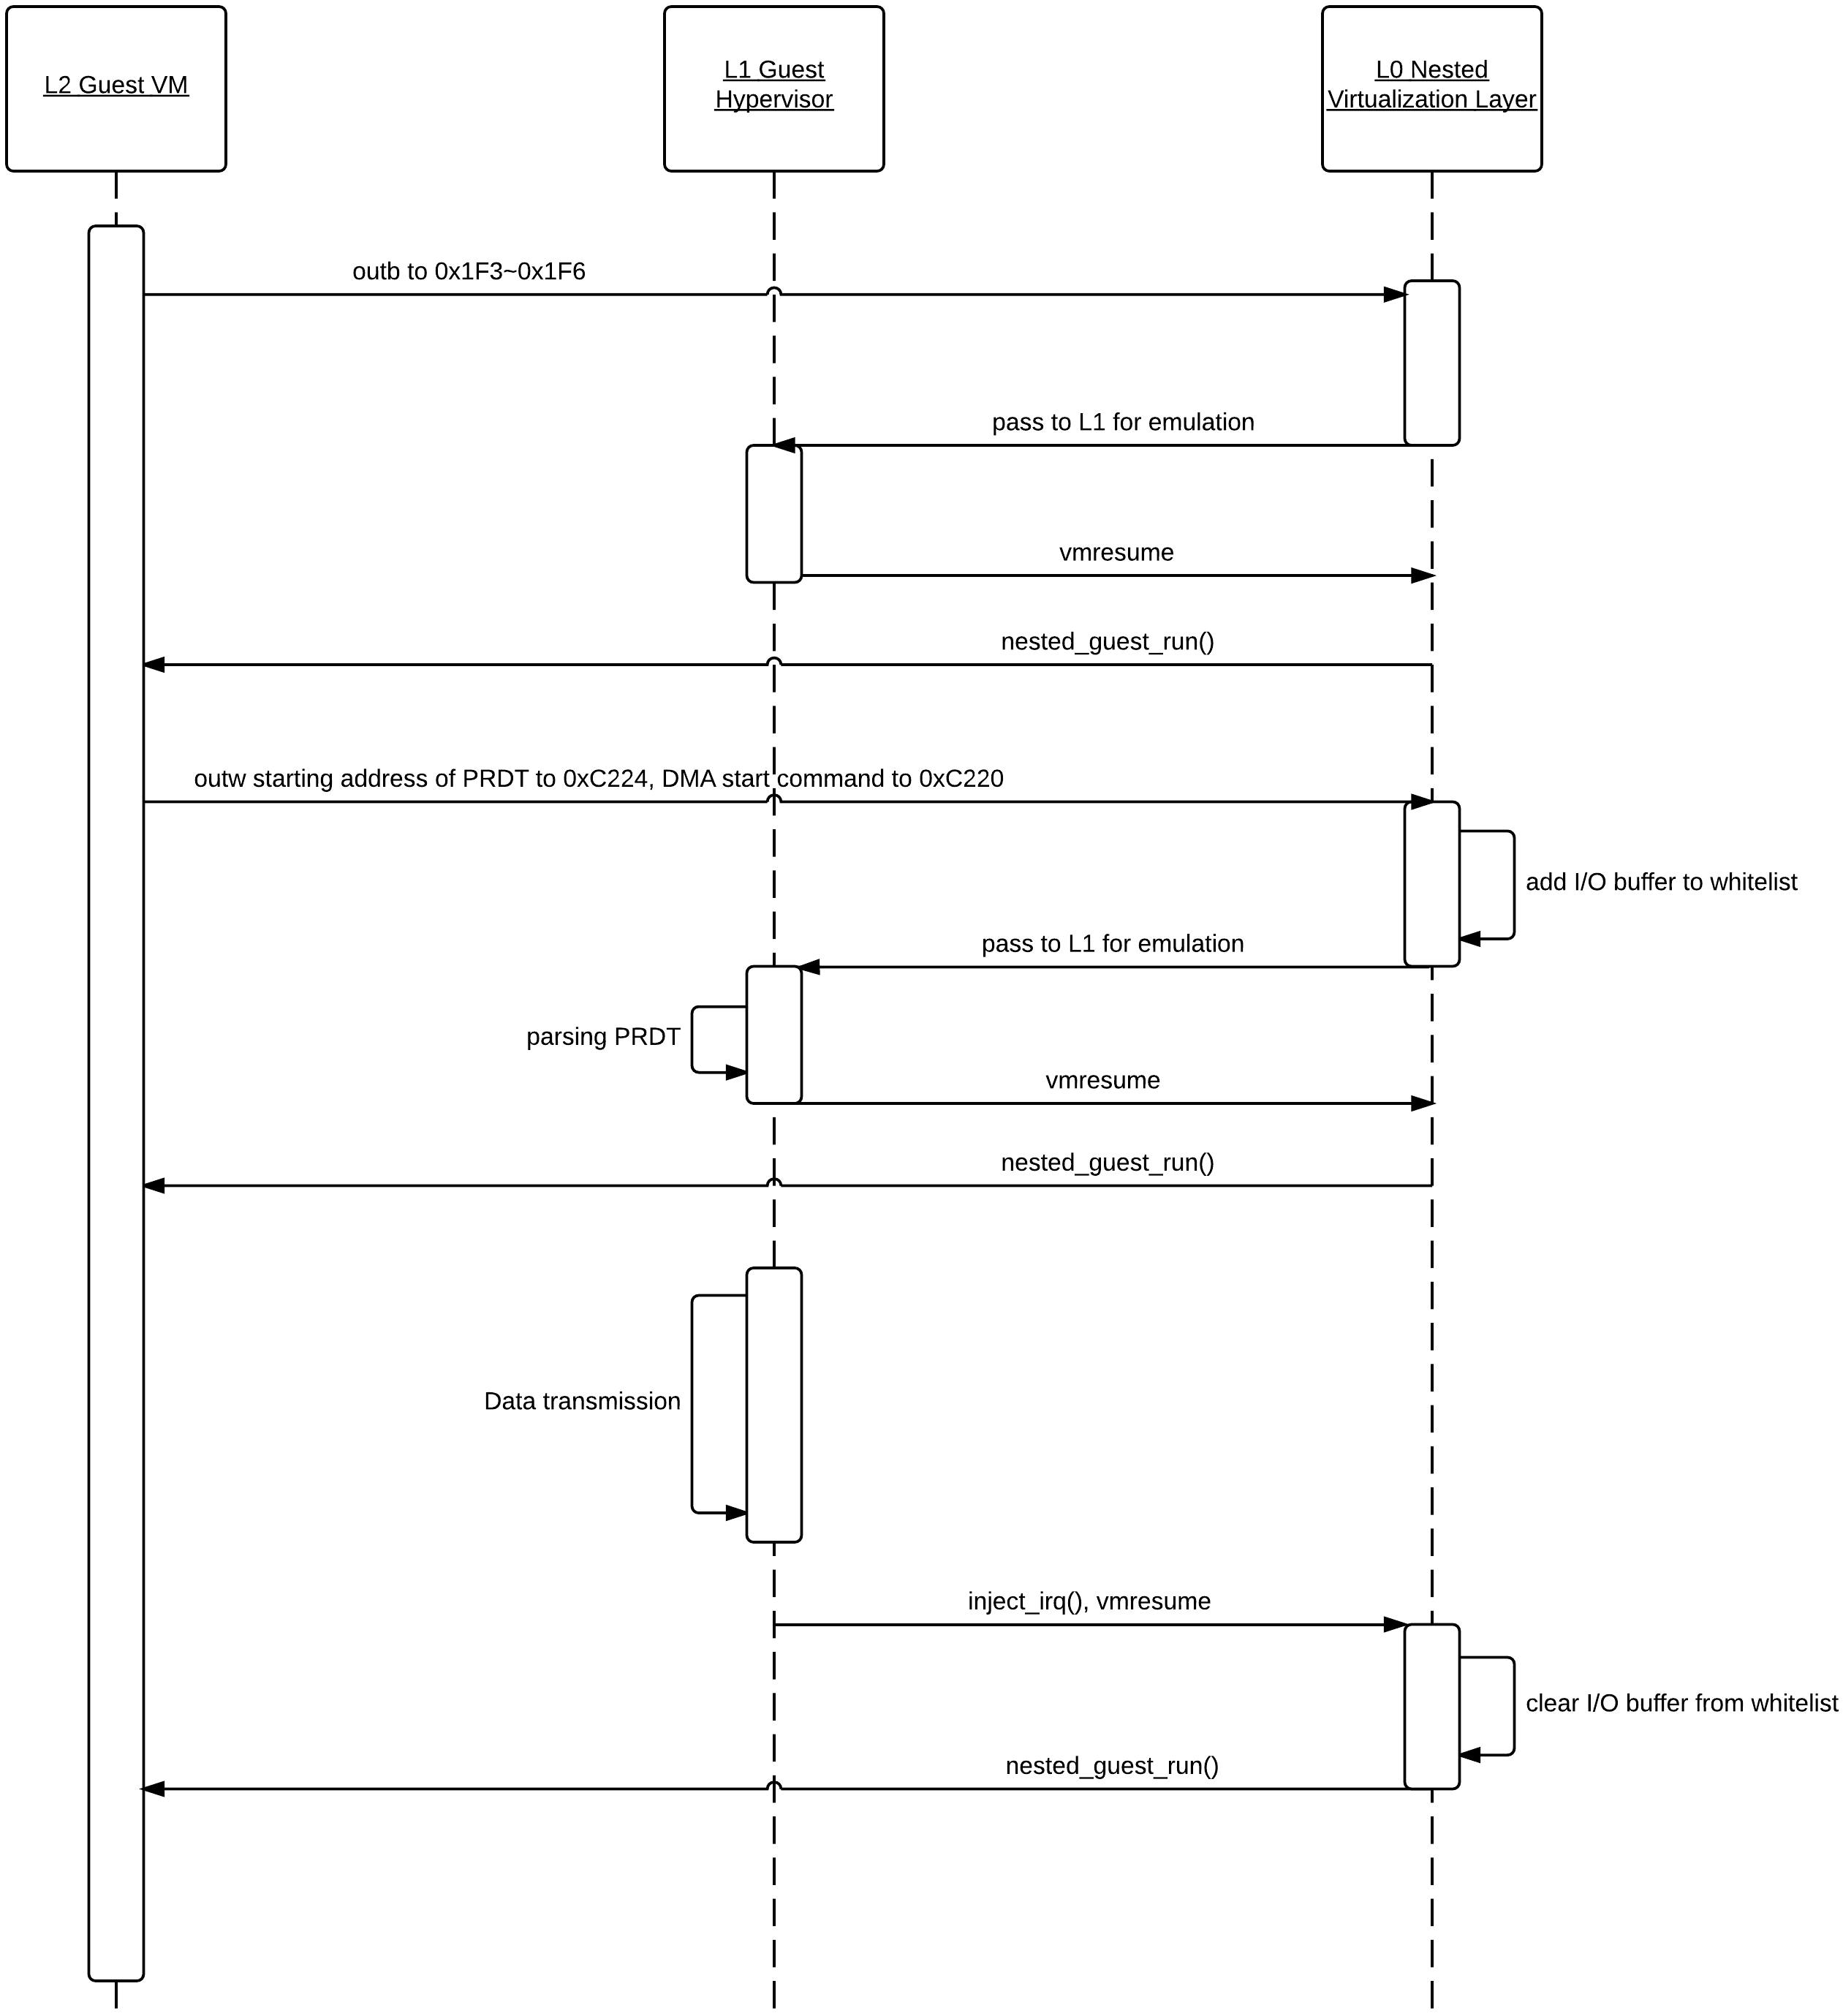
\includegraphics[width=0.95\textwidth]{chap3/dma_read2.png}
  \bicaption[fig:dma_read2]{DMA读取之内存保护顺序图}{DMA读取之内存保护顺序图}{Fig}{Sequence Diagram of memory protection on DMA Read}
\end{figure}

DMA写和DMA读非常相似,只不过L2客户虚拟机会事先准备好待写数据放在内存缓冲区,等待L1将这部分数据写回到磁盘映像中(出于不能在原地址进行加密的原因,L0会将待写磁盘数据拷贝至蹦床缓冲区并对应修改PRDT表,不过这对于L1来说并无任何区别)。在DMA写结束时,L1同样会向L2注入虚拟设备中断,即DMA写在过程开始和结束时都会有相应的事件作为明确界限,L0可以依据此对L1能访问的内存范围做出调整。以上过程的顺序图和DMA读十分相似,此处不再赘述。

\subsection{指令模拟部分的特殊处理}

由于L1在模拟执行L2的某些敏感指令过程中需要访问一些L2的内存,Secure KVM系统需要临时允许L1访问L2敏感指令相关的内存,其中主要涉及到三部分的内存区域。

\begin{enumerate}
\item 敏感指令本身所在的内存页面,L1要模拟这条指令必须先获取其内容。一条x86指令的最大长度为15字节,有可能跨越内存页面边界,这种情况下则是两个内存页面。
\item 页表所在内存页。L1起初获取的一般是x86指令所在的虚拟线性地址,需要经过L2当前页表的翻译才能转化为物理地址(L2 GPA),L1在模拟处理器翻译地址的过程中需要访问L2当前使用的页表页。
\item 在模拟指令执行效果时需要访问的内存页面。如MOV指令需要往某个内存地址写入若干字节数据,这个内存地址对应的页面和地址翻译过程中经历的页表页需要被允许访问。
\end{enumerate}

第一部分内存区域可以由L2客户虚拟机当前RIP、CS等寄存器计算得到。第二部分内存区域可以由L2当前CR3寄存器加载的页表根地址逐级计算得到。第三部分内存区域需要L0对每类敏感指令逐一进行分析,分门别类确定应该被放入白名单中的内存页面。

Intel在其定义的虚拟化扩展中,并没有专门为指令模拟指定一种虚拟化陷入原因(VMExit reason),L1会根据具体问题进行具体分析在需要的情况下进行指令模拟,因此当L2发生虚拟化陷入执行流回到L0时,L0凭借有限的信息不足以判断L1接下来是否要进行指令模拟。出于以上原因,指令模拟部分产生的白名单被设计成惰性的,即每次L0截获L2发生的虚拟化陷入后,先分析当前指令产生白名单但不立即将此白名单添加至EPT01表,如果在接下来L1处理此次虚拟化陷入时需要进行指令模拟,再准许此过程中L1发生的缺页故障陷入并在EPT01表中添加白名单信息,

当L1处理完L2的虚拟化陷入,执行流即将恢复至L2时,L1必定也已经完成了必要的指令模拟,此时正是惰性白名单失效的时候。L0会将上次L2发生虚拟化陷入时产生的白名单销毁,并清除在EPT01表中惰性添加的表项。

由于受到处理器硬件特性限制,对内存数据的保护只能以页大小为粒度,即4KB。在处理指令模拟这种特殊情况时,L2不可避免要向L1暴露多余的内存数据。对于第一部分内存区域而言,当中存放的是程序指令,而在Linux中应用程序数据和指令一般不会存放于同一内存页面(.text段和.data段均为按页对齐),且需要L1为之进行指令模拟的一般是操作系统内核代码,故产生隐私数据泄露的可能性较小。对于第二部分内存区域,页表页本身并不包含隐私数据,其中存放的仅仅是一些地址映射关系。对于第三部分内存区域,由于要模拟的指令一般属于内核,指令执行时本身需要访问的内存页面一般也属于内核,故发生隐私数据泄露的可能性也较小。

\subsection{内存隔离与越界访问检测}
Secure KVM系统利用struct page中的private字段来记录相关内存页面的属主信息。在Linux中每个内存页面都对应着一个struct page,其中记录着该页面的一些基本信息,private字段不是很常用(如果该页面被用作内存文件映射,private字段则指向被映射文件对应的address\_space结构体),在这些内存页被分配给客户虚拟机时,private字段是空闲不用的。又因为struct page的大小对于系统来说很敏感,如增加其中的成员变量则系统中数量庞大的page struct每个都要增大,这是一笔不小的开销,且随意增加page struct中的成员变量有可能破坏先前精心设计的高速缓存行对齐结构。因此,Secure KVM系统选择了一个相对讨巧的方法,充分利用了现有page struct中的空闲部分。

private字段属于unsigned long类型,在64位Linux中为8个字节,用来存放属主信息时被分为了两部分,高4字节中放置了固定的魔数(Magic Number)0xDEADBEAF,低4字节如果值为1表示该内存页面属于L1,如果值为2则表示属于L2客户虚拟机。

L2能访问的内存区域受到EPT02表的控制,而EPT02表在一开始是空白的,L2运行过程中发生缺页故障请求时EPT02表会被动态更新,其中必须经历函数set\_spte,作用是更新EPT表项。Secure KVM在set\_spte中设置了钩子,如果发现当前set\_spte正在往EPT02表中添加新页面,则将该内存页面的属主信息标记为L2,并把EPT01表中可能存在的对该页面的引用清除,L1接下来便不能再访问该页面。由于分配给L2的内存页面究根截底还是从L1的内存地址空间中划分,在L2结束运行后,L0会将EPT02表中页面的属主信息重新标记为L1。

L0嵌套式虚拟化层如果发现L1在运行过程中产生了缺页故障请求,而被请求的页面属主信息为L2且未能在白名单中找到对应的页面信息,则说明L1想要非法访问属于L2的内存。L0针对这种情况特意伪造了一个填充了随机数据的页面,并将这个伪造页面在EPT01表中映射给L1。在L2运行结束后,L0会将EPT01表中的伪造映射更正,从而避免了L1访问L2内存空间中的隐私数据。

临时白名单在最多时一般要存放约5000条内存页面信息。为了加快白名单的查找速度,Secure KVM系统中我们将其设计成了类似哈希表的结构,按页框号的末两位进行分类,在每一类中再用双向链表按序存储。在新内存页被加入白名单时,先要确定该页面页框号的末两位,如某页面的页框号末两位为0x34,则该页面将被放置到第0x34号链表中,并按页框号大小排序。

此外,为了避免处理器TLB缓存过期的白名单信息,L0每次清理白名单中的过期页面数据时都要使用INVEPT指令对TLB进行刷新。

\section{对客户虚拟机磁盘数据的安全保护}

\subsection{基本原理}

在正常的磁盘虚拟化过程中,磁盘读取即是虚拟机监控器将被请求的磁盘数据块从磁盘映像中取出并放置到客户虚拟机指定的内存位置。反之,磁盘写入则是虚拟机监控器从客户虚拟机指定内存位置获取待写数据并存储到磁盘映像相应位置。

由于L2客户虚拟机的设备IO部分仍由L1虚拟机监控器来模拟,L1负责L2实际磁盘IO数据的读取和保存,L2的RAW磁盘映像亦被存储在L1,完全绕过L1不让其接触L2的磁盘IO数据是不实际的。而我们又要保护L2磁盘IO的安全性,故只能退而求其次,让L1始终只能接触到L2加密后的磁盘IO数据。在加密密钥没有被泄露给L1的前提下,加过密的磁盘IO数据对于L1是没有意义的。

要做到这一点,以下四个条件必须得到满足:

\begin{itemize}
\item{L1中存储的L2客户虚拟机磁盘映像必须事先经过加密。否则,L1可以直接以静态方式挂载访问L2磁盘分区和文件系统中的内容。}
\item{当L2进行磁盘读取时,加密后的L2磁盘数据必须要在L1将其读取到相应L2内存空间之后和L2实际使用这一部分数据之前,得到解密。且解密后的这部分数据存在的L2内存空间,L1是被禁止访问的。}
\item{当L2进行磁盘写入时,原先的明文L2待写磁盘数据必须要在L1能接触到其并将其写入磁盘映像之前,得到加密。也就是说,待写磁盘数据在被加密前,其所存在的L2内存空间,L1是被禁止访问的。}
\item{以上三个条件必须做到对L2完全透明,对L1基本透明(L1其实可以发现其上保存的L2磁盘映像是经过加密的)。}
\end{itemize}

对于第一个条件,我们可以用现有的成熟加解密方案处理L2磁盘映像,如AES和DES。

对于第二和第三个条件,L0可以为之完成相应的加解密工作,也可以限制L1对L2的访存范围(通过上节论述)。这里隐含的一个条件是,L0必须能够及时地获取执行机会,也就是说,在需要L0进行加解密时L0必须要得到及时通知。万幸的是,L2客户虚拟机在进行磁盘读取和写入时,均包含了一些敏感操作(IO指令或读写MMIO地址),会立即产生到L0的虚拟机陷入(VMExit),从而让L0得到通知。

对于第四个条件,L2始终接触到的均是明文数据,其不会觉察到L0和L1在事关其磁盘数据安全上做出的斗争。对于L1,除了观察到磁盘映像经过加密这一事实外,在其不威胁L2磁盘数据安全的前提下,其所经历的行为也和正常磁盘虚拟化过程无二致。


\subsection{PIO读部分的处理}

在L2客户操作系统刚启动时,其通过PIO(Programmed Input/Output)的方式读取磁盘数据。PIO是一种同步的简单磁盘数据访问方式。x86处理器上有256个IO端口,其中的一部分被预留给了IDE控制器,如下表所示。而处理器通过x86 ISA中的IO指令(in、out、ins、outs)来读写这些IO端口,来达到访问磁盘数据的目的。PIO的过程是同步的,处理器在执行这些IO指令时不能进行其他工作。待真正进行数据读取的ins(或带req指令前缀的ins指令)执行结束后,磁盘数据即存在于内存中的对应地址。

\begin{table}[htpb]
\bicaption[tab:pio]{磁盘PIO对IO端口的使用说明}{磁盘PIO对IO端口的使用说明}{Table}{x86 IO Port Used in Disk PIO}
\centering
\begin{tabular}{ccc}
\toprule
IO端口号	& 功能 & 描述\\
\midrule
0x1F0	& 数据端口	& 在此端口读写PIO磁盘数据\\
0x1F1	& 特性/错误信息	& 经常被用于ATAPI设备\\
0x1F2	& 扇区数	& 欲操作的扇区数目(0为特殊值)\\
0x1F3	& 扇区号/LBAlo	& 部分扇区地址,取决于寻址方式\\
0x1F4	& 柱面号低位/LBAmid	& 部分扇区地址\\
0x1F5	& 柱面号高位/LBAhi	& 部分扇区地址\\
0x1F6	& 驱动器号/磁头号	& 用于选择驱动器或磁头\\
0x1F7	& 命令端口/状态信息	& 用于发送命令或读取当前状态\\
\bottomrule
\end{tabular}
\end{table}

以下是一个典型的PIO读数据过程。L2先进行IDE主盘/从盘选择,并将之与扇区逻辑块地址(LBA,Logical Block Addressing)高4位作或运算,写入0x1F6端口。随后,L2向0x1F1中写入一个零字节,向0x1F2中写入待读取扇区的数量,并把剩余的LBA地址部分分段写入至0x1F3$\sim$0x1F5。待地址和长度信息写入完毕后,L2向命令端口0x1F7发出读数据指示并轮询等待设备就绪,最后执行rep ins指令接收磁盘数据。

\begin{enumerate}
\item 如果选择是主盘,发送0xE0,如果是从盘,则发送0xF0,并和LBA线性地址的高4位做或运算,结果发送至0x1F6端口:outb(0x1F6, 0xE0 | (slavebit << 4) | ((LBA >> 24) \& 0x0F))
\item 发送一个空字节至0x1F1端口:outb(0x1F1, 0x00)
\item 发送待读取扇区数量至0x1F2端口:outb(0x1F2, (unsigned char) count)
\item 发送LBA线性地址的低8位至0x1F3端口:outb(0x1F3, (unsigned char) LBA))
\item 发送LBA线性地址接下来的8位至0x1F4端口:outb(0x1F4, (unsigned char)(LBA >> 8))
\item 发送LBA线性地址接下来的8位至0x1F5端口:outb(0x1F5, (unsigned char)(LBA >> 16))
\item 发送``扇区读取''指令(0x20)至0x1F7端口:outb(0x1F7, 0x20)
\item 等待来自IDE控制器的中断或进行轮询
\item 从0x1F0端口传输256个机器字至内存缓冲区,每次传输一个机器字(使用带REP前缀的INSW指令)
\item 回到步骤7重新等待中断或进行轮询,此循环对每个后继扇区适用
\end{enumerate}

在非嵌套式虚拟化环境下,每条IO指令均会引发VMExit,最终执行流会转移至Qemu并由其对这些IO指令进行模拟。Qemu对除最后一条rep ins指令外的其他IO指令,均只做简单的簿记工作。到了最后的rep ins指令时,Qemu会根据之前记录的扇区地址和数量信息,从磁盘映像对应位置用pread读出数据并写入虚拟机内存空间对应位置,最后Qemu会调整虚拟机指令指针寄存器rip的数值以恢复虚拟机从下一条指令执行。

由于存放在L1原虚拟机监控器中的L2磁盘映像是经过加密的,L1向L2内存空间中写入的PIO磁盘数据便也是以密文形式存在。为了让L2客户虚拟机正常运行,我们必须适时地对密文PIO磁盘数据进行解密。这个数据解密的时机,便在L1向L2内存空间写入数据后正要恢复L2执行时。这时,待读取磁盘数据已经完整存在于L2内存空间而L2还未能访问这部分数据,且L1用来恢复L2执行的vmresume指令会产生到L0嵌套式虚拟化层的陷入。此过程用UML顺序图可以表示如下。

\begin{figure}[!htbp]
  \centering
  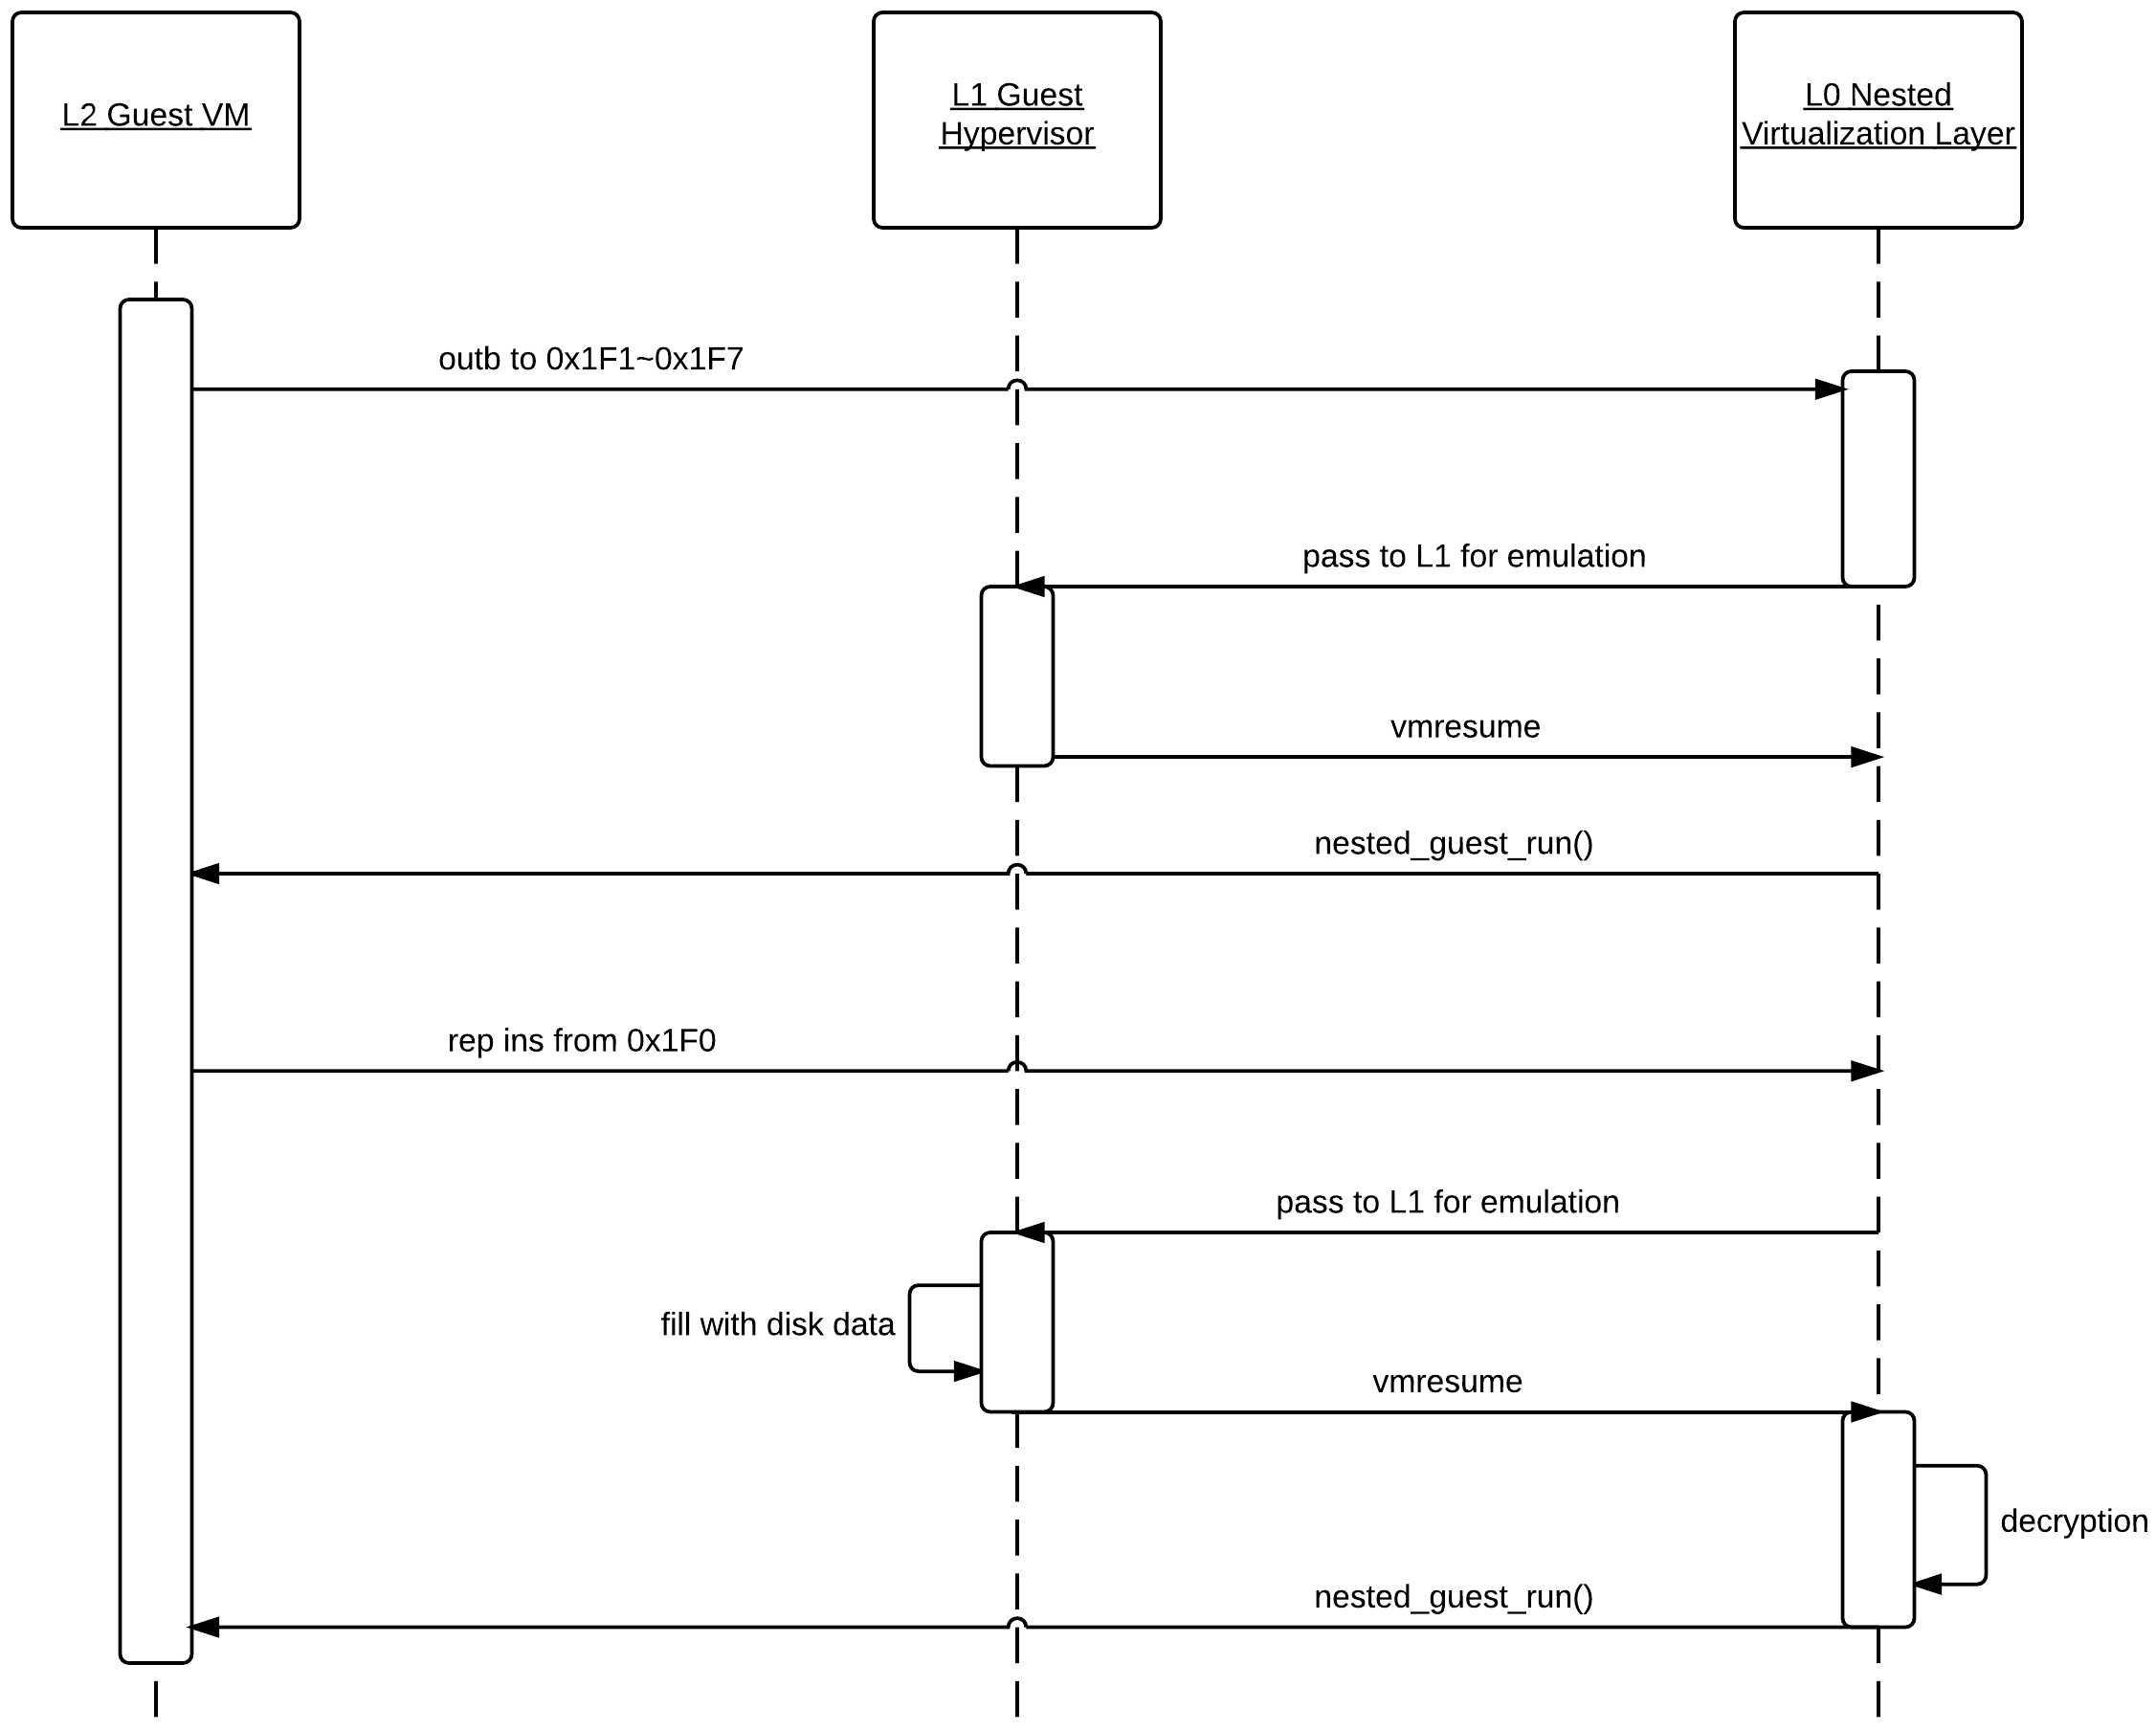
\includegraphics[width=0.95\textwidth]{chap3/pio_read.png}
  \bicaption[fig:pio_read]{PIO读取之解密顺序图}{PIO读取之解密顺序图}{Fig}{Sequence Diagram of decryption on PIO Read}
\end{figure}

L2客户虚拟机进行PIO磁盘读取的粒度是8个磁盘扇区,即每次读取连续的8个普通磁盘扇区,正好是一个对齐的内存页(512B * 8 = 4KB)。L0对其进行解密的过程即为将对应的存放加密磁盘数据的内存页面映射到自己的地址空间,然后用事先约定好的密钥在原地址进行解密操作,其中所涉及到的多层内存地址转换、加解密算法等细节问题将在接下来的章节中进行详细论述。

此外,在原型系统的开发过程中,于PIO层面,我们仅发现有读取行为而未发现磁盘写入。我们猜测PIO读取仅用于Linux初期启动过程中grub将操作系统内核等必要数据载入客户虚拟机内存,待到Linux启动完成后,所有的磁盘操作将转由效率更高的DMA来进行,这部分的论述将在接下来的两节中完成。

\subsection{DMA读部分的处理}

在L2客户虚拟机操作系统加载并初始化完毕后,通过PIO从磁盘读取数据的方式便不再被使用,此时的磁盘操作将转由DMA方式进行。DMA读是一个异步的过程,处理器先将待读取磁盘扇区的信息用IO指令的方式通知IDE控制器(此部分数据的传输与PIO类似),随后再传输描述存放待读取数据缓冲区内存地址的数据结构并发出DMA指令。IDE控制器收到指令后,利用系统总线的空闲期在后台传输读取到的磁盘数据并写入内存缓冲区,在此过程中无需处理器的参与,处理器在此阶段可以继续执行其他指令。等到数据传输完毕后,IDE控制器再向处理器发送特定中断,通知其数据读取已经完成。

\begin{figure}[!htbp]
  \centering
  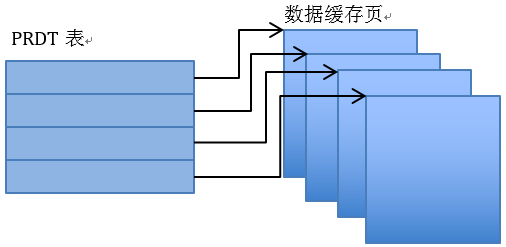
\includegraphics[width=0.75\textwidth]{chap3/prdt.png}
  \bicaption[fig:prdt]{PRDT表示意图}{PRDT表示意图}{Fig}{Illustration on PRDT}
\end{figure}

描述存放待读取数据缓冲区内存地址的数据结构被称作物理区域描述符表(Physical Region Descriptors Table,PRDT)。PRDT中的每个表项大小为8个字节,0-3字节说明内存页面的物理地址,4-7字节说明内存区域的大小,以字节为单位,全零表示64K字节。PRDT表最后一个表项第7字节的最高一位如果被置上则表示PRDT表的结束。之所以要使用PRDT表作为描述内存缓冲区的数据结构,是因为很难从低端内存中找到物理上连续的大块区域(只有低端内存,即物理地址低于32MB的内存空间,能被一般DMA设备访问)。PRDT表实际上是从逻辑角度将多块较小的物理上不连续的内存区域拼凑出了一块虚拟的大块内存区域,类似于集散序列(scatter-gather list)。

\begin{table}[htpb]
\bicaption[tab:dma]{磁盘DMA对IO端口的使用说明}{磁盘DMA对IO端口的使用说明}{Table}{x86 IO Port Used in Disk DMA}
\centering
%\resizebox{\textwidth}{!}{
\begin{tabular}{cc}
\toprule
IO端口号	& 功能描述\\
\midrule
0xC220	&DMA命令端口(一字节)\\
0xC222	&DMA状态端口(一字节)\\
0xC224$\sim$0xC227 &PRDT表基地址(四字节)\\
\bottomrule
\end{tabular}
%}
\end{table}

以下是一个典型的DMA读数据过程。

\begin{enumerate}
\item 磁盘驱动通过写地址为0x1f3$\sim$0x1f6的IO端口,告知IDE控制器待读取磁盘扇区的位置。

\item 磁盘驱动准备好一个PRDT表放在内存中,每个表项8字节,对齐到4字节边界。

\item 磁盘驱动通过写地址为0xc224的IO端口把PRDT表的起始地址设置好,同时通过设置读/写控制位设置数据和传输方向,清除状态寄存器中的中断位和错误位。

\item 磁盘驱动通过写地址为0xc220的IO端口发出DMA传送指令到IDE控制器。

\item 磁盘驱动向总线控制器IDE命令寄存器的对应通道中写入1,使能总线控制器。

\item DMA从磁盘设备中请求IDE控制器传送数据到/从内存中。

\item 数据传送结束,IDE控制器向处理器发出中断。

\item 接收到中断后,磁盘驱动设置命令寄存器的开始/结束位,然后先后读控制器状态、驱动状态,进而确定数据是否传送成功。
\end{enumerate}

由于存放在L1原虚拟机监控器中的L2磁盘映像是经过加密的,L1向L2内存空间中写入的DMA磁盘数据便也是以密文形式存在。为了让L2客户虚拟机正常运行,我们必须适时地对密文DMA磁盘数据进行解密。从以上DMA读数据过程可以看出,IDE控制器中断的到来预示着缓冲区磁盘数据的就绪,客户虚拟机仅可能在接收到虚拟中断后读取缓冲区中的磁盘数据。因此,L1原虚拟机监控器在向L2客户虚拟机注入IDE控制器虚拟中断时,待读取磁盘数据已经完整存在于L2内存空间而L2还未能访问这部分数据,此正好是L0嵌套式虚拟化层解密磁盘数据的时机。此过程用UML顺序图可以表示如下。

\begin{figure}[!htbp]
  \centering
  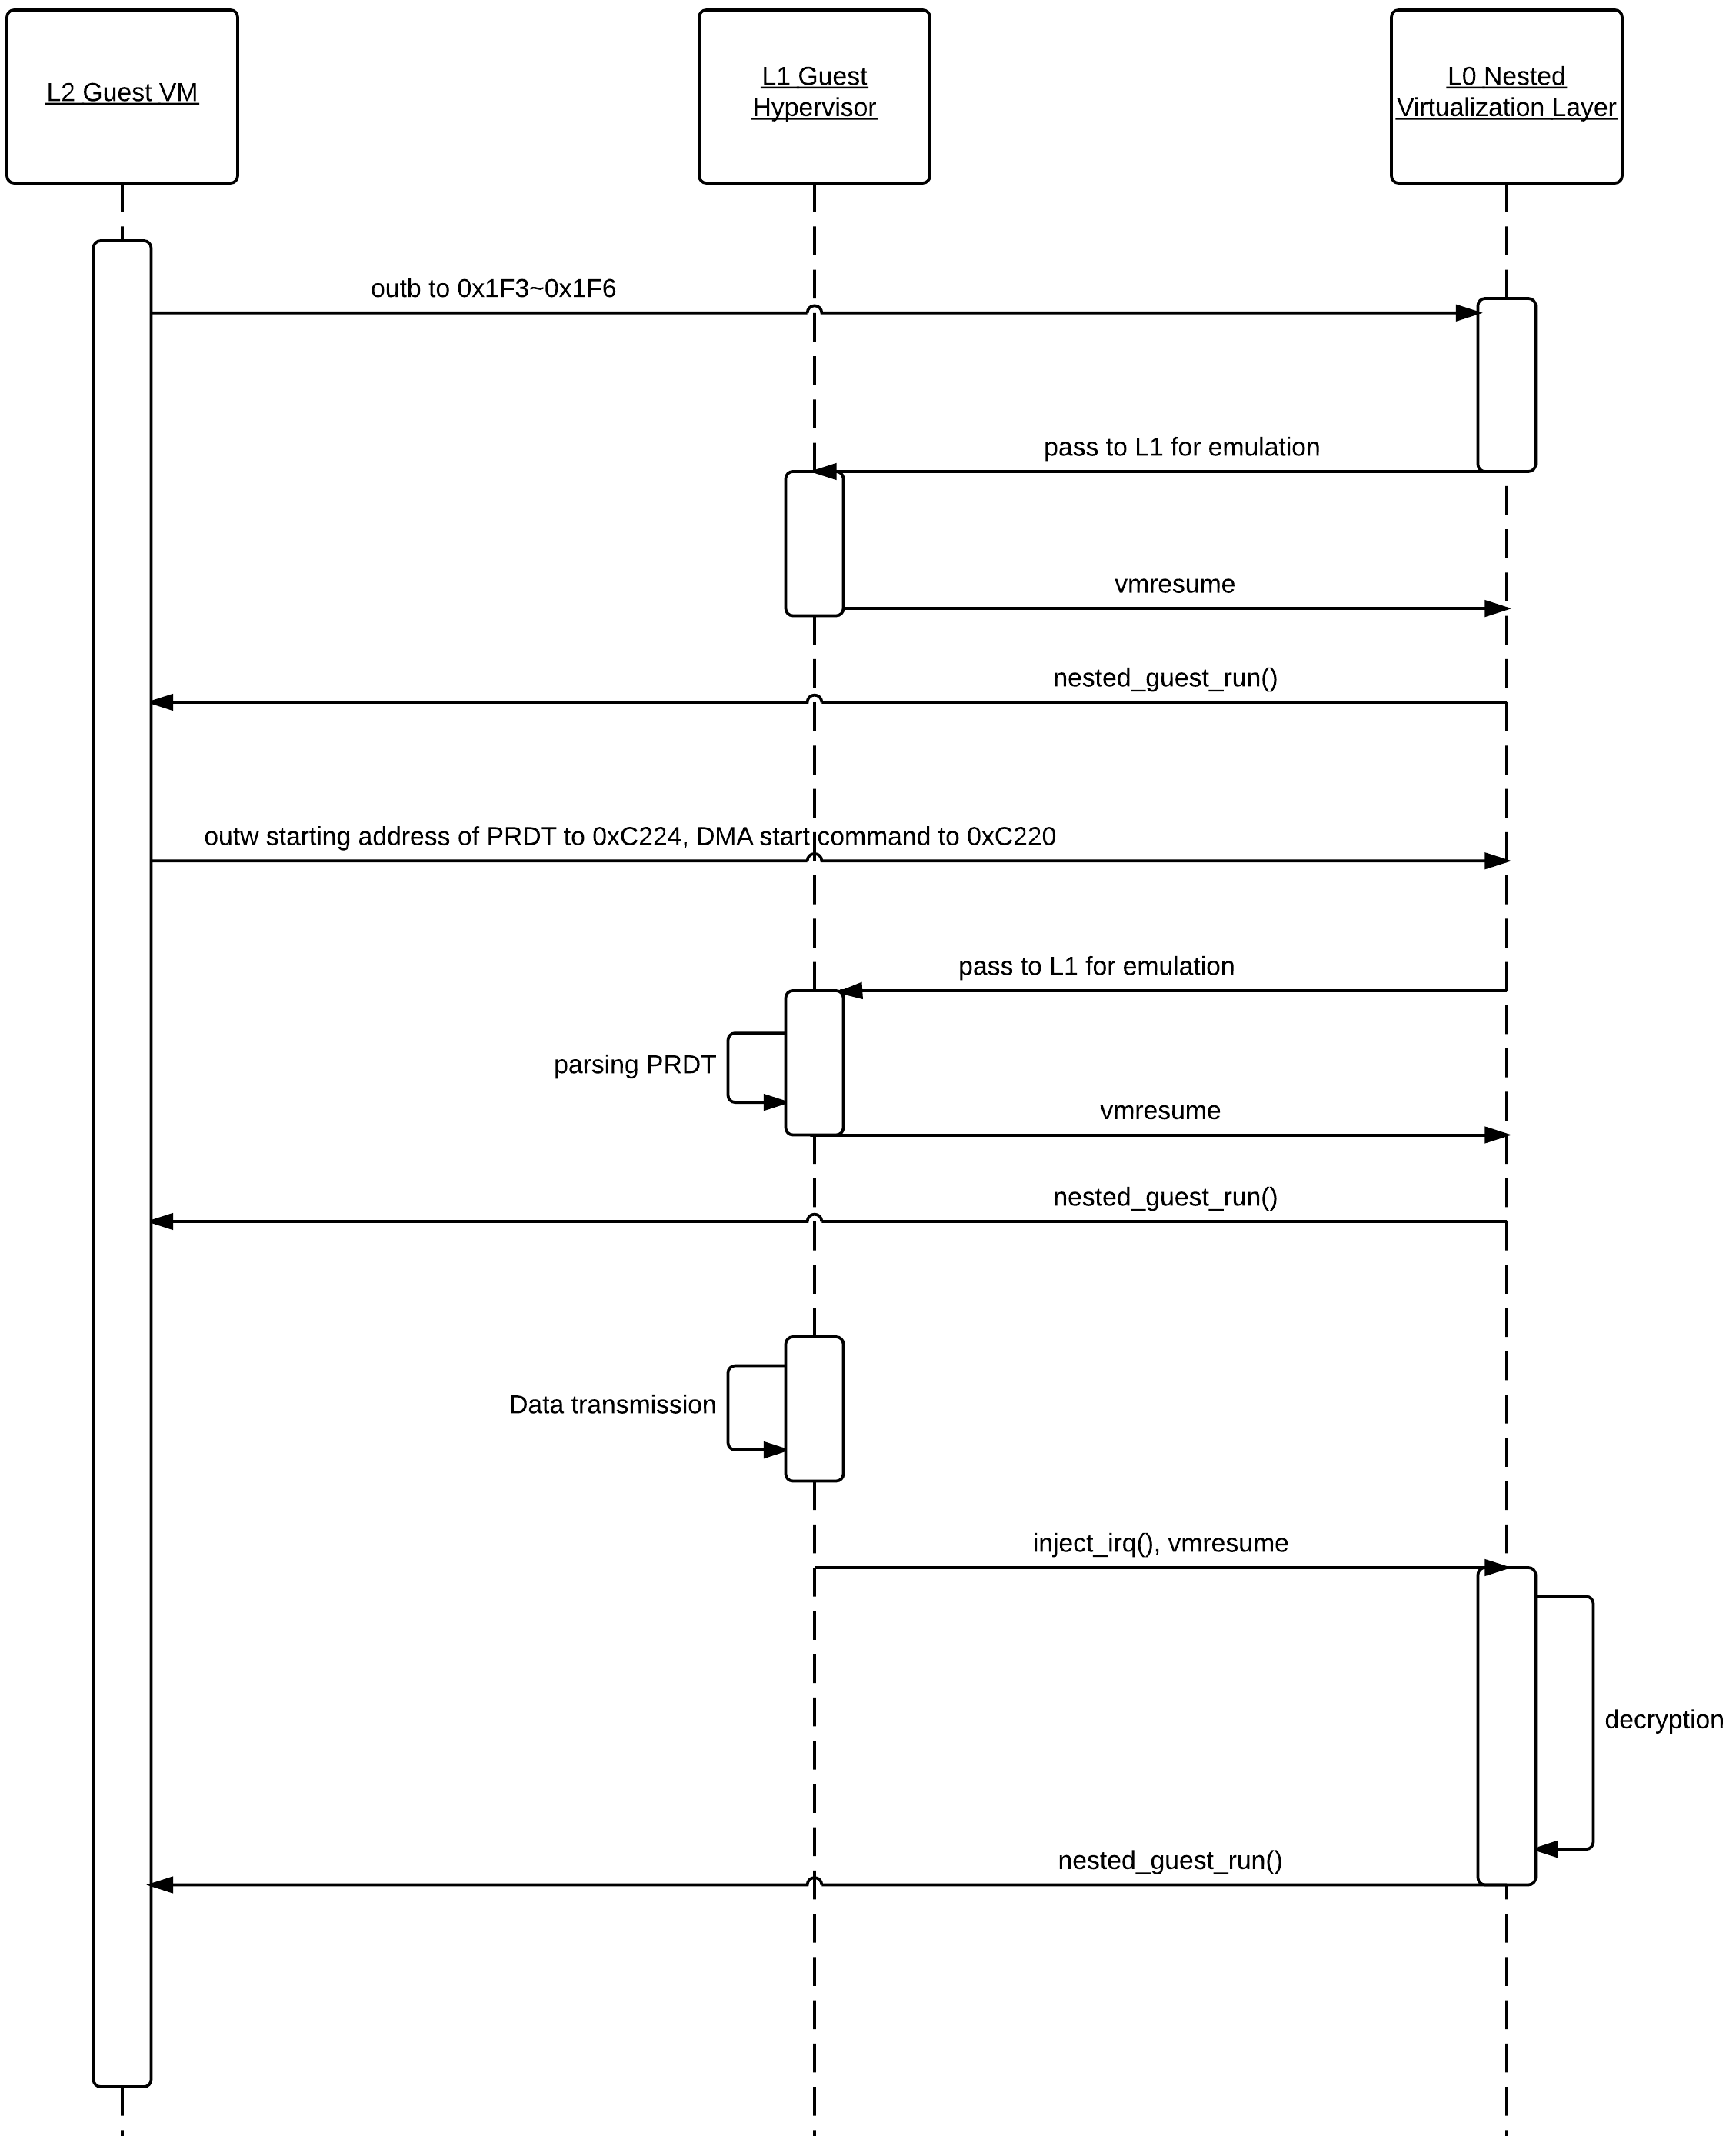
\includegraphics[width=0.95\textwidth]{chap3/dma_read.png}
  \bicaption[fig:dma_read]{DMA读取之解密顺序图}{DMA读取之解密顺序图}{Fig}{Sequence Diagram of decryption on DMA Read}
\end{figure}

在Secure KVM系统的实现过程中,我们发现PRDT表每个表项均以内存页为粒度对齐,即所指向内存区域的起始地址和大小都是4KB的整数倍。L0剩余的工作,就是将这些用作缓冲区的内存页面映射到自己的地址空间,并在原址对其进行解密。其中所涉及到的多层内存地址转换、加解密算法等细节问题将在接下来的章节中进行详细论述。

DMA读取解密过程中还涉及到两个细节问题,分别是识别L2赋予IDE控制器的中断号和检测来自L1的中断注入。因为在DMA读取解密过程中,IDE控制器的中断被作为缓冲区数据是否准备就绪的唯一标志,L0仅可以在检测到相应中断后才能对缓冲区中的磁盘数据进行解密。

L0通过监视L2对PCI配置空间的读写来获取L2赋予IDE控制器的中断号。IDE控制器作为一种PCI设备,在PCI总线上有着固定的地址(总线号、设备号和功能号)。在L2操作系统初始化过程中,其会通过固定的IO端口0xcf8、0xcfc对系统中所有的PCI设备进行配置,并将为设备分配的中断号告知。L0在截取到对应PCI配置空间数据后,即可获得L2为IDE控制器分配的中断号。

检测来自L1中断注入的原理与以上流程类似。L0在检测到L2发出DMA读请求后会为之维护一个上下文环境,里面记录了当前DMA读请求中涉及到的所有信息。当每次执行流从L1回到L0时,L0会检测L1维护的VMCS12中中断相关的字段是否被置位,如VM\_ENTRY\_INTR\_INFO\_FIELD。如果VMCS12中相关字段被置位且被注入的中断向量号相符,L0可以认为当前DMA读请求已经完成,此时应该开始对缓冲区数据进行解密。

\subsection{DMA写部分的处理}

DMA写涉及到的流程和DMA读非常相近。磁盘驱动事先准备好待写入的磁盘数据和PRDT表,然后发出DMA写指令。IDE控制器在将数据转移到磁盘对应位置后,用中断通知处理器DMA写已经完成。

虽然DMA写和DMA读在本身流程上有诸多类似,L0在应对L2客户虚拟机的DMA写请求时做出的保护工作却要复杂繁琐得多。从本质上来说,L0采取这些保护措施的根本目的是为了保证待写磁盘数据在被L1接触到之前得到加密,即禁止L1对明文磁盘数据的访问。但是,如果L0在检测到L2发出DMA写指令后直接在原地址对缓冲区数据进行加密,L2客户虚拟机在恢复运行后不久便会崩溃。其中原因在于,现代操作系统为了提高磁盘访问效率,默认都采取了缓存策略,即将内存的一部分作为磁盘IO的缓存区并用高效数据结构进行管理,如Linux中的页缓存(page cache)。这样一来,之前从磁盘中读取的内容都保存在内存中,等到下次再要用到这部分数据时便可以直接从内存中获得,而根据程序运行的局部性原理,这部分磁盘数据在接下来被用到的概率是很大的。操作系统有时还会采取激进的预读取策略,即把当前没有被请求但处于待读取区域周围的数据预先载入内存。因此,如果L0在原地址对这部分磁盘数据进行加密,L2接下来在运行中便可能读到错误的数据,造成系统崩溃便也不足为奇了。

既然不能在原地址上进行加密,一种直白的解决方案便是拷贝待加密数据到新地址,并在新地址上对磁盘数据进行加密,我们把这种方案称为蹦床缓冲区(trampoline buffer)。此方案的关键之处在于要在L2内存地址空间中寻找一块足够大的且空闲不用的区域。第一个要求为足够大,是因为一个PRDT表中指定的作为磁盘缓冲区的内存页一般有10$\sim$50个之多,约为40$\sim$200KB,用作蹦床缓冲区内存区域的大小必须超过其上限。第二个要求为空闲不用,是因为蹦床缓冲区的存在要对L2客户虚拟机保持透明。

第一种蹦床缓冲区的选取方法是利用L2物理地址空间0KB$\sim$640KB的区域。这部分内存区域在Linux启动过程初期被用来装载grub代码,由于其后方至物理地址为1MB的区域中存在内存空洞(一部分地址被用作MMIO),所以在Linux启动完成后,出于物理内存管理方便考虑,这一小部分内存区域是被弃置不用的。另外,这部分内存区域长度也超过一次DMA写所用到的缓冲区大小上限,正适合被用作蹦床缓冲区。

第二种蹦床缓冲区的选取方法是在L0中监视L2客户虚拟机进行E820内存探测的过程,故意保留一小段内存区,欺骗L2客户虚拟机这部分保留区域是不可访问的,事实上却将这部分内存区域留作他用。

第三种蹦床缓冲区的选取方法是在L2客户虚拟机的Linux启动选项中加入maxmem=255MB(分配给L2客户虚拟机的总内存大小为256MB),这样Linux便不会使用高于255MB的物理内存,L0可以将物理地址空间末端的1MB区域用作蹦床缓冲区。此方法的缺陷是没有让蹦床缓冲区做到对L2客户虚拟机透明,但在万不得已的情况下仍是一种可行方案。

具备了蹦床缓冲区,L0在检测到L2发出DMA写指令后,就会把待写磁盘数据从原地址顺次拷贝到蹦床缓冲区并进行加密,然后再依次修改PRDT表中的各个表项使之对应到新的缓冲区地址,最后再将执行流交还至L1。L1会将加密后的磁盘数据写回L2磁盘映像,在这整个过程中,L1始终没有接触过明文磁盘数据,L2磁盘数据的安全由此得到了保障。

另一种解决不能在原地址上进行加密的方案是对L1的访存行为进行干预。L0在检测到L2发出DMA写指令后,立即在EPT01中去除L1对于存放待写磁盘数据内存区域的读取权限。如此一来,L1中一旦执行对这部分内存区域的访存指令便会产生到L0嵌套式虚拟化层的陷入,L0再借助于指令模拟将加密磁盘数据逐字节地提供给L1。在监测到L1进行IDE控制器中断注入后,L0再在EPT01中恢复L1对于该内存区域的读取权限。这种方案在理论上是可行的,但频繁的由访存指令引发的虚拟化陷入会对性能造成十分严重的影响,故我们在Secure KVM系统的实现中采用了前一种方案,并选取L2物理地址空间底端640KB部分作为蹦床缓冲区。

\subsection{多层内存地址转换的处理}

在嵌套式虚拟化环境下,各层内存地址之间的转化关系尤为复杂,其中经常涉及到的内存地址有以下几种。

\begin{enumerate}
\item L2 GVA,即L2 Guest Virtual Address,L2客户虚拟机中的线性虚拟地址,L2中的应用程序和操作系统内核使用此地址访问内存
\item L2 GPA,即L2 Guest Physical Address,L2客户虚拟机中的物理地址,可以由L2 GVA通过页表转换得到
\item L1 GPA,即L1 Guest Physical Address,L1虚拟机监控器中的物理地址
\item L0 HVA,即L0 Host Virtual Address,L0嵌套式虚拟化层中的线性虚拟地址,L0通过此地址来访问机器上所有的内存空间
\item L0 HPA,即L0 Host Physical Address,L0嵌套式虚拟化层中的物理地址或机器地址,可以由L0 GVA通过页表转换得到
\end{enumerate}

在如此多种内存地址中间,又有若干种页表(或辅助扩展页表)来控制它们之间的转换关系,如图\ref{fig:paging}所示。

\begin{enumerate}
\item L2 PT,负责L2 GVA到L2 GPA的转换,由L2负责维护
\item L1 EPT12,负责L2 GPA到L1 GPA的转换,由L1负责维护
\item L0 EPT01,负责L1 GPA到L0 HPA的转换,由L0负责维护
\item L0 EPT02,负责L2 GPA到L0 HPA的转换,由L0负责维护
\item L0 PT,负责L0 HVA到L0 HPA的转换,由L0负责维护
\end{enumerate}

从逻辑上来说,L2客户虚拟机运行时存在着三层地址转换关系,L2 GVA到L2 GPA的转换,L2 GPA到L1 GPA的转换,和L1 GPA到L0 HPA的转换。但是,CPU在硬件上仅仅支持两层地址转换关系,即普通页表和辅助扩展页表。因此,L0嵌套式虚拟化层需要对后面两层地址转换关系进行压缩合并,在L2客户虚拟机运行时CPU实际使用的辅助扩展页表是EPT02。

\begin{figure}[!htbp]
  \centering
  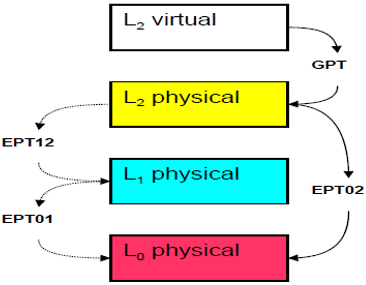
\includegraphics[width=0.7\textwidth]{chap3/paging.png}
  \bicaption[fig:paging]{多层内存地址转换示意}{多层内存地址转换示意}{Fig}{Illustration on Multi-dimensional Paging}
\end{figure}

在L0嵌套式虚拟化层进行磁盘数据加解密时,必须适时地进行内存地址之间的转换。如负责L2 GPA到L1 GPA转换的EPT12表,其根地址和表项中的地址数据均以L1 GPA的形式存在。又如L2客户虚拟机进行DMA操作时使用的PRDT表,其中的表项地址数据以L2 GPA的形式存在。下文将以L2 GPA到L0 HVA为例,详述其中的地址转换过程。

L0先去EPT02中查找L2 GPA到L0 HPA的对应关系,此功能由ept02\_p2m函数实现。ept02\_p2m先从当前VMCS中读出EPT02表的根地址,然后模拟硬件查表行为,将L2 GPA划分为4段并分别去索引EPT表的每一级。如EPT02表中每一级表项都存在且合法,ept02\_p2m将返回转换后的L0 HPA,否则ept02\_p2m将返回0表示此次尝试失败。

\begin{lstlisting}[language={C}, caption={ept02\_p2m实现源代码}]
static unsigned long ept02_p2m(unsigned long pfn) {
    unsigned long ept_hpa = vmcs_readl(EPT_POINTER);
    int l4i, l3i, l2i, l1i;
    unsigned long mfn;
    ept_entry_t *ept_hvm, *cur_epte, *l2_epte;

    ept_hvm = (ept_entry_t*)pfn_to_kaddr(ept_hpa >> PAGE_SHIFT);

    l4i = (pfn >> 27) & 0x1ff;
    l3i = (pfn >> 18) & 0x1ff;
    l2i = (pfn >> 9) & 0x1ff;
    l1i = pfn & 0x1ff;

    /* L4 */
    cur_epte = ept_hvm + l4i;
    if (!(cur_epte->epte & 0x7)) {
        return 0;
    }
    
    /* L3 */
    cur_epte = (ept_entry_t*)(pfn_to_kaddr(cur_epte->mfn)) + l3i;
    if (!(cur_epte->epte & 0x7)) {
        return 0;
    }
    if (cur_epte->sp_avail) {
    	/* 1G super page */
        mfn = cur_epte->mfn + (pfn & 0x3ffff);
        return mfn;
    }

    /* L2 */
    ......
    /* L1 */
    ......

    mfn = cur_epte->mfn;
    return mfn;
}
\end{lstlisting}

但是在KVM中,为了节省内存开销,EPT表采用按需填充(populate on demand)的方式进行更新,即EPT在客户虚拟机刚启动时仅为一张空表,其中内容只有等到页错误发生时才会被增添或修改。这个特性会给内存地址转换带来问题,使得EPT02中的地址映射关系可能是不完整的,因为此时L2客户虚拟机很有可能还没有访问过这部分内存页,这些L2 GPA在EPT02表中的对应项是空缺的。

如果发现EPT02中有表项缺失的情况,L0会模拟EPT02表的构建过程,从EPT01和EPT12中读取原始数据并进行合并,从而构造出L2 GPA到L0 HPA的转换关系。从EPT01和EPT12中读取数据的过程和ept02\_p2m类似,此处不再赘述。

有了L2 GPA对应的L0 HPA,L0可以使用pfn\_to\_kaddr等功能函数将其再转化为线性虚拟地址,便可以对该内存区域进行访问。

\subsection{缺失内存地址转换的处理}

在大部分情况下,直接从EPT02表中获取L2 GPA到L0 HPA的映射关系,或者退而求其次,从EPT01和EPT12中的数据整合出L2 GPA到L0 HPA的映射关系,是满足要求的。但在某些极端情况下,这种方式仍然会产生问题。

现假设L2客户虚拟机发起了一次DMA读数据请求,并在PRDT表中指定物理地址(L2 GPA)为0x12345000$\sim$0x12346000的内存区域作为数据缓冲区。但是,L2尚未访问过这部分内存区域,所以EPT02表中不会存在到L0 HPA的映射关系。同理,EPT12表中也不会存在到L1 GPA的映射关系(EPT01表中可能存在L1 GPA到L0 HPA的映射关系,取决于此时L1有无将磁盘数据填入缓冲区),此时便不能取得L2 GPA到L0 HPA的映射关系,无法对原先加密的磁盘数据进行解密。

有两种方案可以被用来解决该困境,分别为主动式和被动式。

主动式解决方案在发现内存地址转换缺失时,通过向L1注入虚拟缺页故障,来诱使L1填补EPT12表。待到执行流从L1返回后,EPT12表中便已存在L2 GPA到L1 GPA的映射关系,此时再将其与EPT01表中的数据合并,便可以获取L2 GPA到L0 HPA的映射关系。以上过程在inject\_virtual\_ept\_fault函数中实现。

\begin{lstlisting}[language={C}, caption={inject\_virtual\_ept\_fault实现源代码}]
static int vmx_handle_exit(struct kvm_vcpu *vcpu) {
	......

    if (is_guest_mode(vcpu) && vmx->inject_virtual_ept_fault) {
        inject_virtual_ept_fault();
        return 1;
    }

	......
}

static void inject_virtual_ept_fault() {	
    struct vmcs12* vmcs12;
    struct dma_entry* dma = NULL;

    /* switch execution flow back to L1 */
    nested_vmx_vmexit(vcpu);
    vmcs12 = get_vmcs12(vcpu);
    dma = (struct dma_entry*)container_of(vcpu->dma_list.next, struct dma_entry, next_entry);

    /* fake an ept violation */
    vmcs12->vm_exit_reason = EXIT_REASON_EPT_VIOLATION;
    vmcs12->exit_qualification = 0x0000000000000003;
    vmcs12->guest_physical_address = dma->dma_addr;

    vmx->inject_virtual_ept_fault = 0;
}
\end{lstlisting}

在L0处理虚拟机陷入的函数vmx\_handle\_exit中,一旦发现vmx->inject\_vi\-rtual\_ept\_fault标志位被设置,便会调用inject\_virtual\_ept\_fault向L1中注入虚拟缺页故障。inject\_virtual\_ept\_fault首先调用nested\_vmx\_vmexit让L1在处理器下次进入非根模式时获得运行机会。由于在嵌套式虚拟化环境下,L0对于L1是透明的,L1在重新获得运行机会后会认为是L2发生了虚拟机陷入,便会从VMCS12中读取陷入的原因并进行相应处理。因此,inject\_virtual\_ept\_fault还必须在VMCS12中模拟出陷入现场,这是通过设置VMCS12中的三个关键字段vm\_exit\_reason、exit\_qualification和guest\_physical\_address(即L2 GPA)来达到。最后,inject\_virtual\_ept\_fault清除虚拟缺页故障注入标志位,L1继续运行并填补EPT12表中空缺的映射关系。

另一种方案是通过被动方式来解决该问题。此方案是基于这样的考虑,L2客户虚拟机要访问磁盘数据,EPT02表中必须要存在相应L2 GPA到L0 HPA的映射关系。因此,我们可以延迟对转换缺失的L2内存区域的解密工作,将其暂存至链表中,并对EPT02表的更新进行监视。一旦,EPT02表中增添了新的映射关系,说明L2即将对这部分内存区域进行访问,此时可以继续之前未完成的数据解密工作,并将已完成解密的内存区域从暂存链表中移除。

我们对以上提及的主动式方案和被动式方案均进行了实现,经过性能测试,发现主动注入虚拟缺页故障的方案性能要远超被动解密方案。这是由于EPT02表的更新是一个进行比较频繁的操作,一旦对其设置了监视,每次EPT02表更新发生时均需要对待解密链表进行遍历。而L2由于操作系统的页缓冲预取策略,不一定会立即访问读取后的磁盘数据,这便会造成待解密链表中经常积累至超过万项的待解密内存页,每次对其进行遍历开销巨大。最终,在Secure KVM系统的实现中,我们采取了主动式方案。

\subsection{加解密方案与数据完整性保护}

Secure KVM系统中采用了AES(Advanced Encryption Standard) ECB算法对L2磁盘映像数据进行加解密。AES在密码学领域又被称为Rijndael加密法,是美国联邦政府采用的一种区块加密标准。AES算法被用来代替先前的DES(Data Encryption Standard),已经被多方分析研究且广为全世界所使用。经过五年的甄选流程,AES由美国国家标准与技术研究院于2001年发布,并在2002年成为有效标准。2006年,AES已然成为对称密钥加密中最流行的算法之一。

存储在L1原虚拟机监控器中的L2客户虚拟机磁盘映像是事先经过AES加密的,且密钥只存在于L0嵌套式虚拟化层中,因此从静态角度来看L1能接触到的仅仅是一个加过密的映像文件,L1甚至都不能获取磁盘映像的分区信息,更谈不上挂载分区获取其中的文件内容。从动态角度来看,L1按照L2发出的磁盘读取请求,从磁盘映像对应位置读取数据,其读到的也是密文数据。当L2发出磁盘写入请求时,在L1能接触到这部分待写入数据前,L0已经对其完成了加密,L1同样不能窥探到明文内容。L2客户虚拟机的磁盘数据安全由此得到保障。

Secure KVM系统中提供了如下接口对一段内存数据进行加解密。

\begin{lstlisting}[language={C}, caption={inject\_virtual\_ept\_fault实现源代码}]
typedef struct {
	......
} RIJNDAEL_context;

int rijndael_setkey(void *context, char *key, int keylen);
void rijndael_encrypt (void *context, unsigned char *out, const unsigned char *in);
void rijndael_decrypt (void *context, unsigned char *out, const unsigned char *in);
\end{lstlisting}

rijndael\_setkey用于设置加解密过程中使用到的密钥,密钥其实是创建L2客户虚拟机时静态生成的一段字节数组,其长度为16个字节。rijndael\_encrypt被用于加密以第三个参数in为起始地址的长度为16字节的内存区域,并将加密后的数据写到第二个参数out所指向的内存区域。相反,rijndael\_decrypt被用来解密数据,其参数数目和意义与rijndael\_encrypt完全相同。

AES ECB算法要求被处理的数据块大小为16字节的整数倍。在PIO读操作中,每次操作涉及到连续的8个磁盘扇区,共计4096字节,可以满足要求。在DMA读取和DMA写入中,每次指定的缓冲区均为若干个完整的内存页面,即4096字节的整数倍,同样可以满足要求。

AESNI(Advanced Encryption Standard New Instructions)是Intel在2008年3月提出的在x86处理器上的指令集扩展,它包含了7条新指令,其中6条是硬件对AES的支持,另1条是对进位乘法的优化,从而在执行 AES 算法的某些复杂的、计算密集型子步骤时更好地利用底层硬件,减少计算消耗的CPU时钟周期,提升AES加解密的性能。Intel从Westmere平台开始就支持AESNI,目前Westmere、SandyBridge、IvyBridge、Haswell等平台都提供对AESNI的支持。

Secure KVM系统在初始化时会检测当前处理器是否支持AESNI,如果支持,rijndael\_encrypt和rijndael\_decrypt中会自动采用该处理器特性以加速加解密流程,如果不支持,rijndael\_encrypt和rijndael\_decrypt中会采用软件方法来模拟实现AES。两者最后得到的加解密结果是完全一致的,仅在速度性能上有50\%左右的差距。

检测处理器是否支持AESNI的功能在detect\_aesni函数中实现,此处借助x86上的CPUID指令来作出判断,返回非0表示支持,返回0表示不支持。

\begin{lstlisting}[language={C}, caption={detect\_aesni实现源代码}]
#define X86_FEATURE_AES_SHIFT	25

static int detect_aesni() {
	unsigned int eax = 1, ebx, ecx, edx;
	__asm__ __volatile__
    (
        "cpuid"
        : "=a" (eax), "=b" (ebx)
        , "=c" (ecx), "=d" (edx)
        : "a"  (eax)
    );
    return ecx & (1 << X86_FEATURE_AES_SHIFT);
}
\end{lstlisting}

L1原虚拟机监控器还能够通过一种可能的途径来威胁L2客户虚拟机的磁盘数据安全,即破坏磁盘数据完整性。具体来说,L1能够控制其写入到L2磁盘缓冲区中的数据,如果L1写入的是一段恶意的随机构造的无意义磁盘数据,虽然L1不能获取明文磁盘数据,其却可以让L2客户虚拟机不能正常运行。

为了应对来自L1磁盘数据完整性威胁,Secure KVM系统在L0中还为每个L2磁盘映像维护了一个对应的元数据文件,这个元数据文件记录了L2磁盘映像每个扇区的MD5哈希值。L0在L2客户虚拟机启动后,会将整个元数据文件载入内存。每次解密磁盘数据之前,L0会对加密磁盘数据先行计算哈希值,并与元数据文件中记载的数值进行比较,如发现不同,便说明L1恶意破坏了磁盘数据完整性,此时最好的做法是终止L1和L2的运行。相反,每次L2发出磁盘写入请求时,L0在对待写入数据进行加密后,会重新计算这部分数据的哈希值,并对元数据文件中的对应区域进行更新。

在Secure KVM系统的实现中,L2客户虚拟机磁盘映像的大小为5GB,对每个磁盘扇区采用MD5算法计算后得到的哈希值是128bit,故元数据文件的最终大小为160MB,在可以接受的大小范围内。

\section{实验与性能测试}

\subsection{实现与配置}

Secure KVM系统中,L0嵌套式虚拟化层采用安装了嵌套式虚拟化补丁的Linux,代码源自KVM开发git库的queue分支,内核版本号为3.10.0-rc1。此外,L1和L2均为未经修改的普通Linux发行版,L1使用了带图形界面的Ubuntu 10.04桌面版本并安装了KVM,L2使用了不带图形界面的Ubuntu 10.04服务器版本。

运行Secure KVM的机器配置如表\ref{tab:machine}所示。

\begin{table}[htpb]
\bicaption[tab:machine]{运行Secure KVM系统的机器配置}{运行Secure KVM系统的机器配置}{Table}{Host Configuration for Secure KVM System}
\centering
\begin{tabular}{cc}
\toprule
配置项	& 规格\\
\midrule
处理器	& Intel Xeon E3-1230 v2 (8M Cache, 3.30 GHz)\\
内存	& 16GB\\
主板	& Gigabyte B75M-D3V\\
\bottomrule
\end{tabular}
\end{table}

Intel Xeon E3-1230 v2处理器提供了第二代硬件辅助虚拟化支持,并支持AESNI指令集扩展。在L1和L2运行过程中,我们分别为其分配了8GB和512MB的内存空间。

在L0中启动L1虚拟机监控器的命令行如下,加入-cpu host配置项是因为要将处理器的硬件特性全部暴露给L1。

qemu-system-x86\_64 -m 8192 -hda ./l1.img -enable-kvm -cpu host

在L1中启动L2客户虚拟机的命令行如下。

qemu-system-x86\_64 -m 512 -hda ./l2.img -enable-kvm

\subsection{内存攻击与防御}

\noindent
\textbf{攻击\uppercase\expandafter{\romannumeral1}}:在虚拟机监控器中窥探客户虚拟机的进程列表和模块列表

LibVMI是一套用于虚拟机自省的工具和应用程序库。LibVMI在虚拟机监控器提供接口的前提下,可以访问运行中的客户虚拟机内存,并提供了用物理地址、虚拟地址和客户操作系统内核函数符号进行访存寻址的命令原语。LibVMI还支持操作客户虚拟机的内存快照,从中获取有用语义信息,对调试和取证分析能起到很大帮助。

LibVMI在examples文件夹下提供了process-list和module-list两个样例程序,分别可以被用于获取客户虚拟机中正运行的进程列表和已加载的内核模块列表。Linux中,所有当前正在运行的进程都在内核地址空间有与之对应的task\_struct结构体,而系统中所有的task\_struct结构体均被双向串联成环状链表,process-list程序通过先找到init\_task这个内核符号地址,并对该环状链表进行遍历,从而获取客户虚拟机中所有的进程信息。module-list程序的运行原理与上述流程类似。图\ref{fig:libvmi:a}和图\ref{fig:libvmi:b}分别显示了process-list和module-list这两个程序在正常普通虚拟化平台之上的运行情况。

\begin{figure}
\centering
\subfigure[process-list的运行结果]{
\label{fig:libvmi:a} %% label for first subfigure
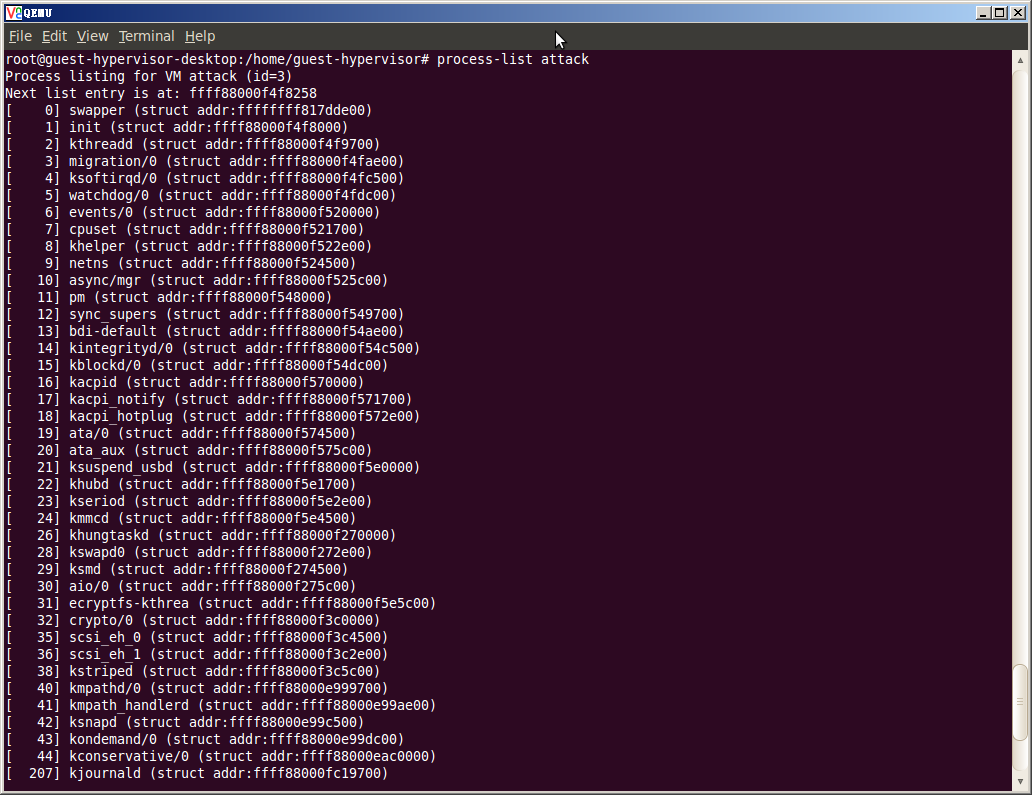
\includegraphics[width=0.8\textwidth]{chap3/process_list_a.png}}
%\hspace{1px}
\subfigure[module-list的运行结果]{
\label{fig:libvmi:b} %% label for second subfigure
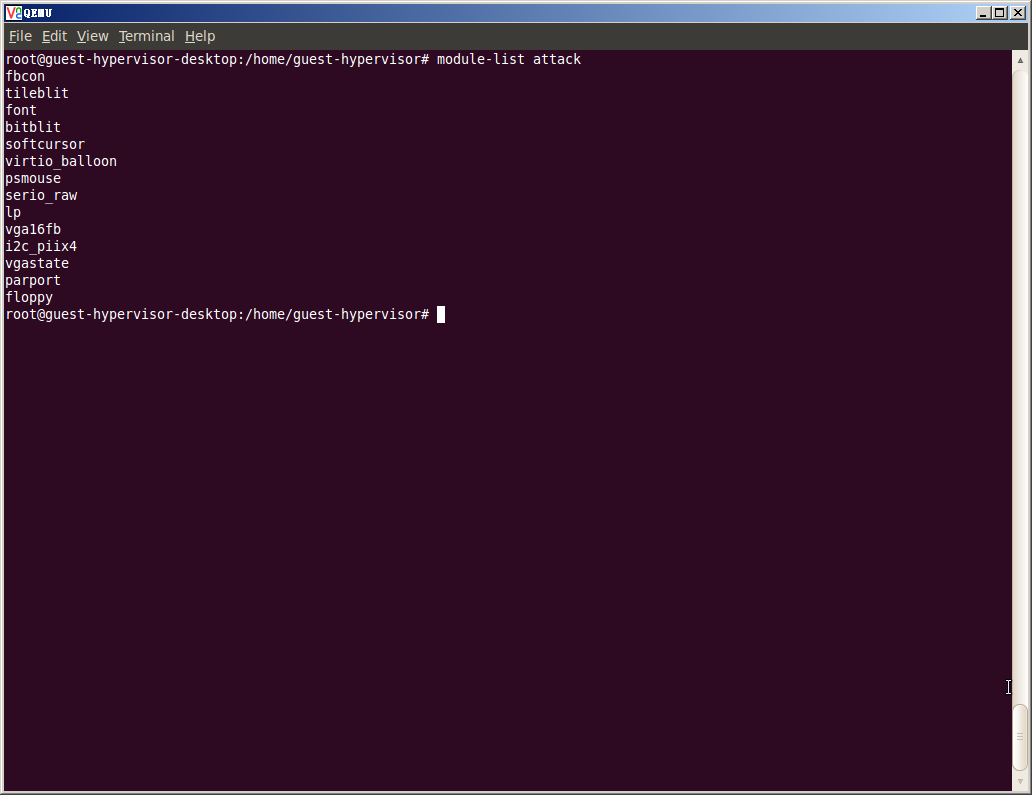
\includegraphics[width=0.8\textwidth]{chap3/module_list_a.png}}
\bicaption[fig:libvmi]{LibVMI示例程序在正常虚拟化平台上的运行结果}{LibVMI示例程序在正常虚拟化平台上的运行结果}{Fig}{Illustration on running results of LibVMI applications on normal virtualization platform}
%\label{fig:libvmi} %% label for entire figure
\end{figure}

之所以process-list和module-list这两个样例程序能获取客户虚拟机的进程信息和模块加载信息,是因为在正常虚拟化平台上虚拟机监控器能轻易获取客户虚拟机所有的内存并访问其中的数据。此行为具有一定的危险性,恶意的虚拟机监控器可以挑选感兴趣的客户进程进行分析,进而访问其进程地址空间,如果这恰好是一个浏览器进程,其进程地址空间中保存的已浏览网页数据和账号密码等信息很有可能因此而被泄露。

\noindent
\textbf{防御\uppercase\expandafter{\romannumeral1}}:阻止L1窥探L2的进程列表和模块列表

在Secure KVM系统中,我们同样在L1虚拟机监控器中运行process-list和module-list两个程序,结果如图\ref{fig:libvmi2}所示。

\begin{figure}[!htbp]
  \centering
  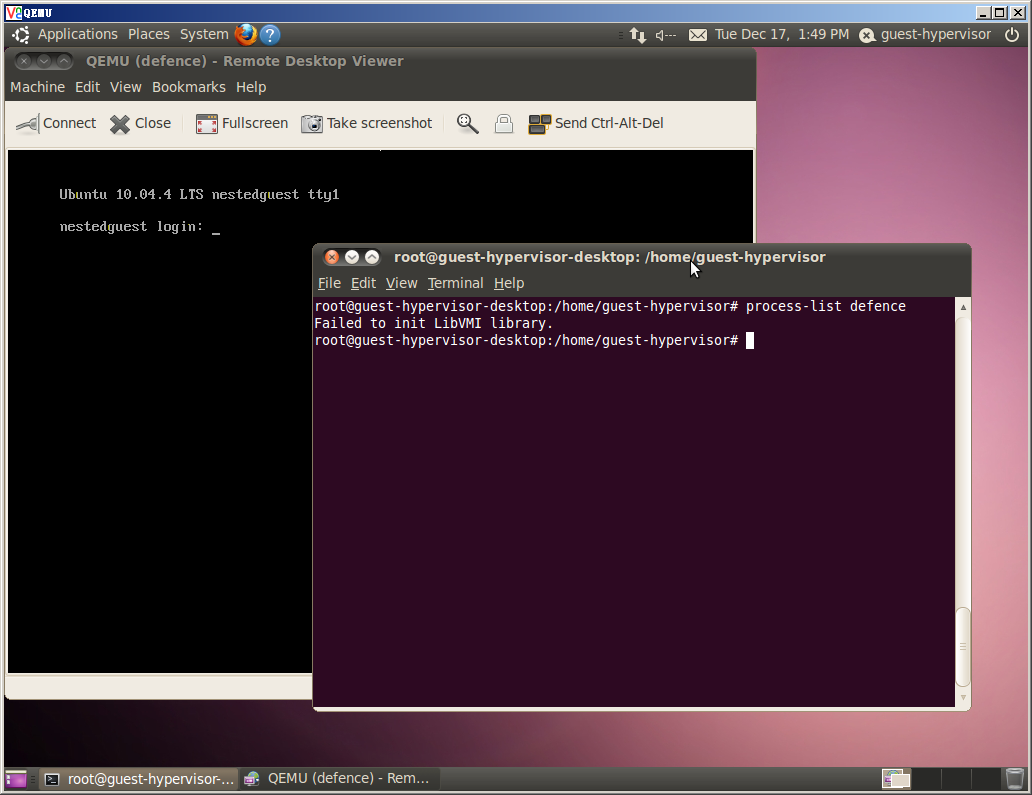
\includegraphics[width=0.8\textwidth]{chap3/process_list_b.png}
  \bicaption[fig:libvmi2]{process-list程序在Secure KVM上的运行结果}{process-list程序在Secure KVM上的运行结果}{Fig}{Illustration on running result of process-list in Secure KVM}
\end{figure}

当L1虚拟机监控器在试图映射属于L2客户虚拟机的内存页面时,此行为会被L0嵌套式虚拟化层检测到,L0会使用一张填充了随机数据的伪造页面来欺骗L1。LibVMI中的样例程序会发现其获取的内存数据不符合预定规则(其实是垃圾随机数据),未能通过规则检查,便会显示结果为``Failed to init LibVMI library''。而此时,L2客户虚拟机仍然在正常运行,其内存中的隐私数据受到了L0的保护。

\noindent
\textbf{攻击\uppercase\expandafter{\romannumeral2}}:客户虚拟机中的普通权限进程提权

Linux操作系统在/etc/shadow文件中保存了系统中所有用户的权限、加密密码等关键信息,正常情况下只有系统管理员即超级用户(uid=0)才有权利进行查看和修改。客户虚拟机中开始时以普通用户权限(uid=1000)运行了root-hijack程序,由于其不具备超级用户权限,root-hijack程序不能访问/etc/shadow文件中的数据。打开/etc/shadow文件时,open系统调用会返回-1,即无用文件描述符,同时会提示EPERM错误信息,即权限不足,如图\ref{fig:root_hijack_a}所示。

\begin{figure}[!htbp]
  \centering
  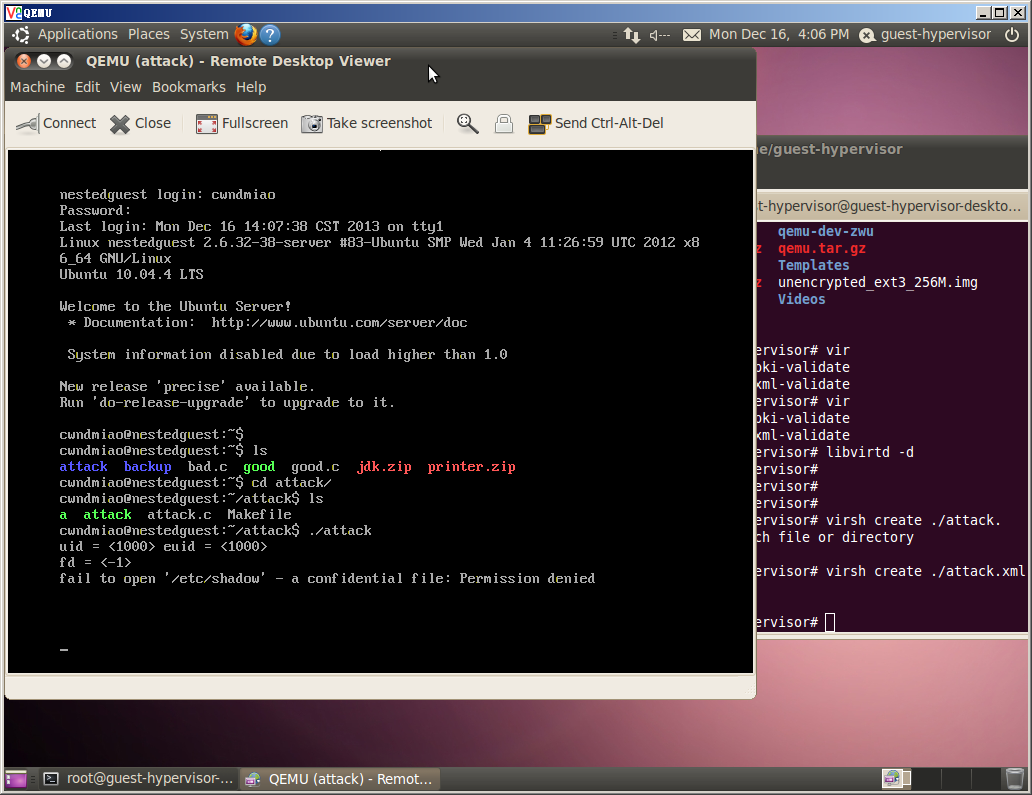
\includegraphics[width=0.8\textwidth]{chap3/root_hijack_a.png}
  \bicaption[fig:root_hijack_a]{root-hijack程序未能读取/etc/shadow文件}{root-hijack程序未能读取/etc/shadow文件}{Fig}{Failure of root-hijack on accessing /etc/shadow}
\end{figure}

此时,在虚拟机监控器中执行修改后的process-list命令,该命令经过修改后能定位root-hijack进程的task\_struct结构体并将该结构体中的uid和euid均替换为0,此时root-hijack进程便在事实上具备了超级用户权限,因为Linux操作系统在系统调用中仅仅简单地根据task\_struct结构体中的数据域来进行权限检查。root-hijack程序经由恶意虚拟机监控器的协助,现在能顺利获取/etc/shadow文件中的隐私数据,除此之外,一切原先需要超级用户权限才能实施的操作均能顺利进行。如图\ref{fig:root_hijack_b}所示。

\begin{figure}[!htbp]
  \centering
  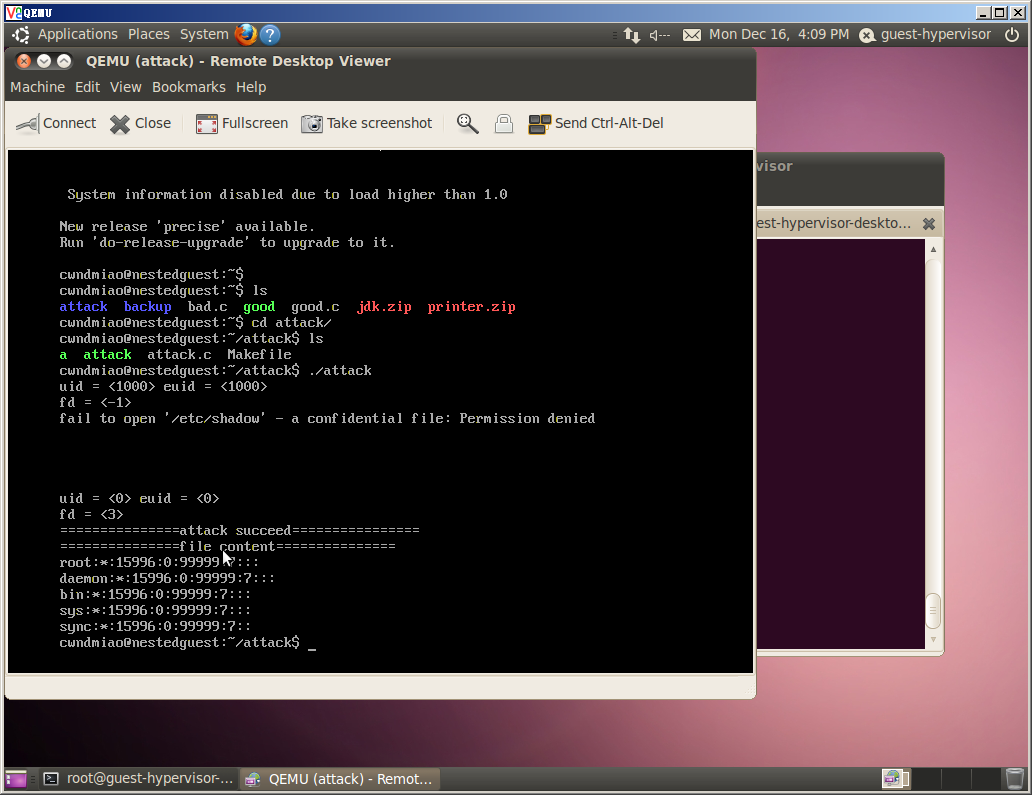
\includegraphics[width=0.8\textwidth]{chap3/root_hijack_b.png}
  \bicaption[fig:root_hijack_b]{root-hijack程序顺利读取/etc/shadow文件}{root-hijack程序顺利读取/etc/shadow文件}{Fig}{Success of root-hijack on accessing /etc/shadow}
\end{figure}

此例为虚拟机监控器在获取系统中进程信息后,有针对地修改客户虚拟机特定内存,帮助普通权限进程提权。此现象存在的根本原因仍在于在普通虚拟化平台上虚拟机监控器能不受控制地任意访问属于客户虚拟机的内存。

\noindent
\textbf{防御\uppercase\expandafter{\romannumeral2}}:阻止L1帮助L2中的普通权限进程提权

在Secure KVM系统中,我们同样在root-hijack程序运行至一半时,于L1中执行修改后的process-list命令。由于L0嵌套式虚拟化层使用了填充了无效数据的内存页去欺骗L1,process-list命令的运行结果仍然如图\ref{fig:libvmi2}一样,L1帮助root-hijack程序提升权限的举动未能成功。

\noindent
\textbf{攻击\uppercase\expandafter{\romannumeral3}}:在虚拟机监控器中改变客户虚拟机中正常程序的执行流

在客户虚拟机中编译并执行名为good的普通程序,good程序本身的行为很简单,在控制台上打印5行``do something good''字符串便退出。然而事实上,good程序的实际执行效果却是与预期大相径庭,在控制台上打印出了5行``do something bad'',如图\ref{fig:exe_flow}所示。

\begin{figure}[!htbp]
  \centering
  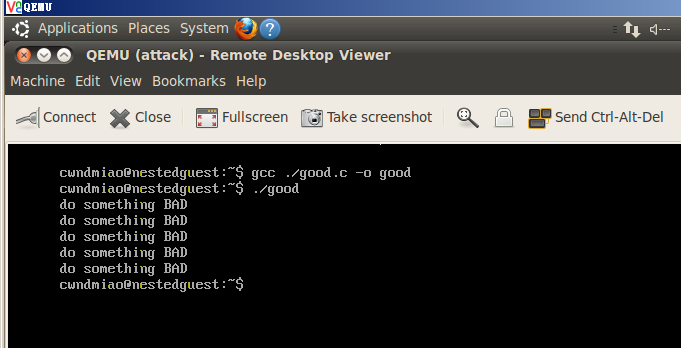
\includegraphics[width=0.8\textwidth]{chap3/exe_flow.png}
  \bicaption[fig:exe_flow]{被执行流劫持后的good程序运行行为}{被执行流劫持后的good程序运行行为}{Fig}{Running results of a hijacked application}
\end{figure}

之所以会出现截然相反的执行结果,是因为L1虚拟机监控器将good程序的.text段部分替换成了一截精心构造的shellcode。这段shellcode的作用是合理设置客户虚拟机的寄存器值,并执行INT 0x80软件中断以发起exec系统调用,执行另一个名为bad的程序,而bad程序的行为是往控制台上打印5行``do something bad''。

此行为对客户虚拟机而言具有较大危险性,事实上bad程序的行为可以是任意的(开启远程shell或格式化磁盘)。例如,攻击者可以通过Web网页上传任意恶意程序至客户虚拟机,再通过此种方式让恶意程序获得执行,便可以完全控制该客户虚拟机。

\noindent
\textbf{防御\uppercase\expandafter{\romannumeral3}}:阻止L1改变L2中正常程序的指令流

在Secure KVM系统中,L1虚拟机监控器不能任意接触L2客户虚拟机的内存,因此L1写shellcode时也仅仅是把这段恶意代码写到了伪造的L2内存页面中。L1在为L2客户虚拟机进行指令模拟时,L0允许L1访问L2被模拟指令所在的内存页面,然而L1对此内存页面仅有读取权限,同样不能达到写入恶意shellcode的目的。具备了L0嵌套式虚拟化层的保护,good程序在Secure KVM系统内的执行行为符合预期。

此外,在L1完成对L2客户虚拟机的指令模拟后,执行流重新回到L0时,L0会对L2关键寄存器的值进行检查(如rip、rflags等,执行流攻击)。如果发现L2关键寄存器的值发生无缘由的改变,L0会认定L1正在对L2进行执行流攻击,L0此时会暂停L1和L2的执行。

\subsection{静态磁盘攻击与防御}

\noindent
\textbf{攻击\uppercase\expandafter{\romannumeral4}}:在虚拟机监控器中挂载客户虚拟机磁盘映像分区并查看修改其中的文件

在普通虚拟化平台上,客户虚拟机的磁盘映像以明文形式存储在虚拟机监控器中。虚拟机监控器可以很容易地查看磁盘映像中的分区信息(在MBR格式的磁盘中,分区信息存储在磁盘的第一个扇区中),并选择特定分区进行挂载。挂载磁盘映像分区后,虚拟机监控器可以任意查看和修改分区内的文件。

一个可能的攻击案例为,虚拟机监控器可以在挂载分区后将虚拟机磁盘映像中的可执行文件替换为恶意程序并为之添加自启动项,等到客户虚拟机启动后,该恶意程序便能获得运行机会。

\noindent
\textbf{防御\uppercase\expandafter{\romannumeral4}}:阻止L1挂载L2磁盘映像分区和查看修改其中的文件

由于存在放L1虚拟机监控器中的L2客户虚拟机磁盘映像已经事先经过了AES加密,L1在无法获取加密密钥的前提下,不能获取磁盘映像的明文内容。L1甚至不能获取L2磁盘映像中的分区信息,挂载分区并修改文件内容更无从谈起。

此外,L0会在客户虚拟机运行时对磁盘数据的完整性进行检查(比对每个扇区的MD5哈希值是否相符),如果L1企图通过恶意修改磁盘映像数据破坏L2正常运行,此行为也能够被L0及时发现。

\subsection{动态磁盘攻击与防御}

\noindent
\textbf{攻击\uppercase\expandafter{\romannumeral5}}:在虚拟机监控器中记录客户虚拟机运行过程中的磁盘活动

客户虚拟机的磁盘设备由Qemu来模拟,恶意虚拟机监控器能够通过修改Qemu,记录客户虚拟机所有的磁盘活动,包括读取和写入磁盘的所有数据。如图\ref{fig:disk_dynamic}所示,在刚开启的客户虚拟机中执行写磁盘操作,如echo ``teststring'' >> test \&\& sync,在修改版Qemu的qemu-disk-attack/disk\_log/目录下即可以看到刚才写入的数据。

\begin{figure}[!htbp]
  \centering
  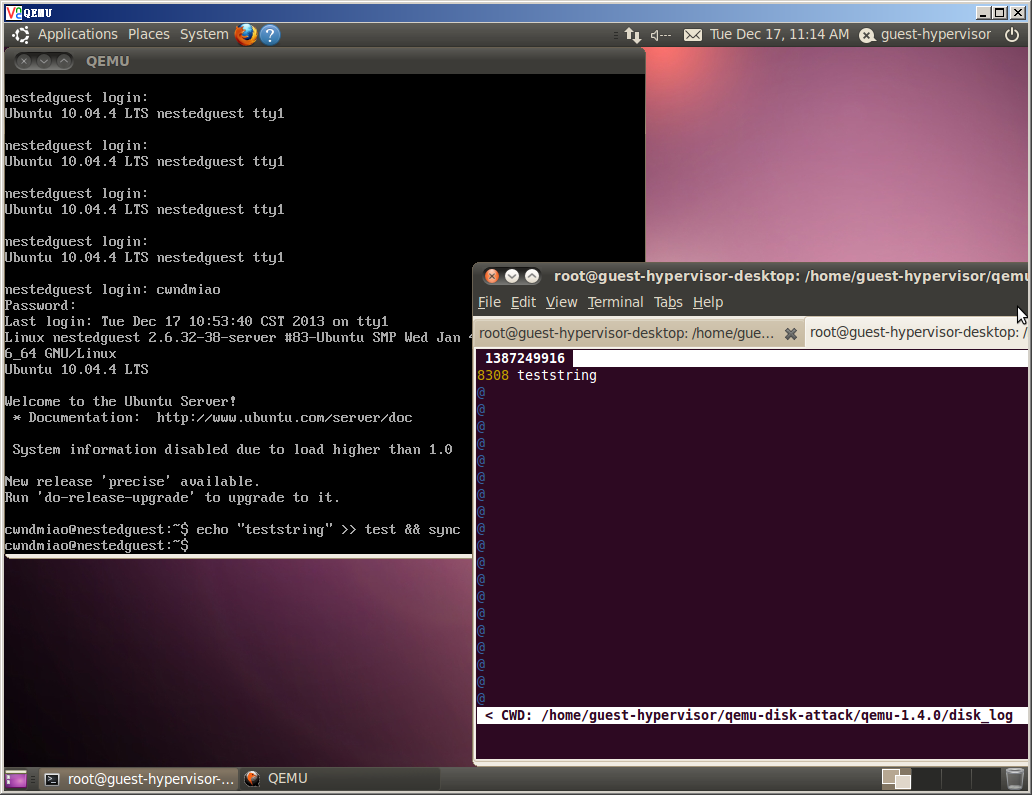
\includegraphics[width=0.8\textwidth]{chap3/disk_dynamic.png}
  \bicaption[fig:disk_dynamic]{通过修改Qemu记录客户虚拟机的磁盘活动}{通过修改Qemu记录客户虚拟机的磁盘活动}{Fig}{Disk operation recording with modified Qemu}
\end{figure}

\noindent
\textbf{防御\uppercase\expandafter{\romannumeral5}}:阻止L1记录L2运行过程中的磁盘活动

在Secure KVM系统中,L0嵌套式虚拟化层在L1接触到待写入的L2磁盘数据之前,会先行对这部分磁盘数据进行加密,此外L1从客户虚拟机磁盘映像中读取并写入L2内存空间的也是密文数据,因此L1始终只能接触到加密后的客户虚拟机磁盘数据。即使L1通过修改版的Qemu对这部分数据进行了记录,对其也没有任何明显意义。

\subsection{性能测试}

% Table generated by Excel2LaTeX from sheet 'Sheet1'
\begin{table}[htbp]
  \centering
  \bicaption[tab:kvm_perf]{Secure KVM系统的性能比较}{Secure KVM系统的性能比较}{Tab}{Performace evaluation of Secure KVM and other platforms}
    \begin{tabular}{ccccc}
    \toprule
          & Native KVM & Nested KVM & Secure KVM \\
    \midrule
    md5sum 100M & 0.238s & 0.886s & 0.906s \\
    md5sum 250M & 0.738s & 3.080s & 3.503s \\
    pi 1000000 > /dev/null & 1.262s & 1.290s & 1.302s \\
    pi 2500000 > /dev/null & 3.773s & 3.853s & 3.859s \\
    pi 5000000 > /dev/null & 8.883s & 9.164s & 9.341s \\
    unzip 100M & 0.768s & 2.694s & 3.579s \\
    unzip 250M & 2.479s & 7.017s & 7.811s \\
    encrypt 100M & 0.798s & 1.772s & 2.070s \\
    encrypt 250M & 2.024s & 4.581s & 5.490s \\
    decrypt 100M & 0.431s & 1.728s & 2.108s \\
    decrypt 250M & 1.070s & 4.490s & 5.509s \\
    \bottomrule
    \end{tabular}%
\end{table}%

表\ref{tab:kvm_perf}比较了应用程序在Secure KVM系统和原生KVM、嵌套式KVM上的运行性能。测试选取了md5sum、pi、unzip和openssl这四个程序,并对每个程序测试了若干种不同大小的数据集。测试结果显示,Secure KVM系统的性能和嵌套式KVM没有太大差别,然而和原生KVM相比有较大下降。

Secure KVM系统中应用程序性能的下降大部分可以归结于嵌套式虚拟化,因为原本虚拟机监控器可以直接接收并处理的虚拟化陷入事件在嵌套式虚拟化中均需要L0代为转发,此外L0对L1行为进行的安全检查以及运行时对磁盘数据的加解密工作也造成了一定的性能开销。


\section{相关研究工作分析}

Secure KVM利用嵌套式虚拟化,获取系统最高权限后监控虚拟机监控器的行为,防止其威胁客户虚拟机的内存和磁盘数据安全。而随着虚拟化技术和多租户云的不断普及,虚拟化平台之上的安全问题正越来越受到开发者、研究人员和社区的关注。

HyperSentry针对虚拟机监控器本身因代码量膨胀而带来的更多隐含漏洞,利用IPMI( Intelligent Platform Management Interface)建立的特殊信道向处理器发出系统管理中断(System Management Interrupt, SMI),并在处理器系统管理模式这个特殊上下文中对虚拟机监控器的行为进行完整性和正确性检查,以便及时发现虚拟机监控器被入侵的迹象,保护虚拟机监控器的安全。

NoHype试图通过在客户虚拟机运行时借助一些新的硬件机制去除虚拟机层来解决多租户云环境中的虚拟机监控器和客户虚拟机间的信任问题。但在去除虚拟化层的同时,NoHype也失去了普通虚拟化带来的一些有用特性,比如多虚拟机之间方便的资源共享。除此之外,NoHype还信任虚拟机管理软件,且需要对现有硬件和软件栈进行较大程度的修改。目前,NoHype系统还不存在完整的实现。

SecVisor在现有操作系统下方添加权限级别更高的较薄虚拟化层,对操作系统内核的行为进行完整性和正确性检查,以确保操作系统运行期间只有用户审查通过的代码可以在内核态执行,以防止针对操作系统内核的代码注入攻击(如内核级rootkit)。

Overshadow与SecVisor实现途径类似,也是在现有操作系统下方添加权限级别更高的较薄虚拟化层,不同的是Overshadow的目的是为了保护应用程序的隐私数据不被操作系统窥视。在Overshadow系统中,应用程序接触与使用资源的方式与普通情况下并无明显差别,而操作系统所能涉及的只能是加密后的内容。

BitVisor针对传统虚拟机监控器因模拟大量虚拟设备和控制硬件资源在客户虚拟机间共享而膨胀的代码量和降低的可靠性,提出了一种新的虚拟机监控器架构。BitVisor允许绝大多数的I/O访问直接穿透虚拟机监控器,将虚拟机监控器从巨量虚拟设备模拟中解脱,同时保护了一些I/O设备访问和数据传输的安全性。

Secure KVM系统和CloudVisor的设计目的类似,均是为了防止恶意虚拟机监控器窥探客户虚拟机中的隐私数据。然而,Secure KVM系统基于KVM实现,而CloudVisor基于Xen实现,两者在实现细节上存在相当的差异。例如,在Xen中分配给客户虚拟机的内存范围在虚拟机启动时便已经确定,而KVM采用按需分配策略在客户虚拟机发出缺页故障请求时才为其分配内存。

\section{本章小结}

本章关注虚拟化环境中客户虚拟机内存和磁盘数据的安全问题。本章先对虚拟化的本质进行了分析,并阐述了恶意虚拟机监控器可能对客户虚拟机进行攻击的方式,提出了一种基于嵌套式虚拟化的解决方案。为了解决内存数据的安全保护问题,Secure KVM系统用辅助扩展页表限制虚拟机监控器的访存范围,并依靠临时白名单部分允许其访问客户虚拟机的指定内存页面。为了解决磁盘数据的安全保护问题,Secure KVM系统对客户虚拟机的磁盘映像进行了加密,并适时地对磁盘操作中涉及到的数据进行加解密,以确保虚拟机监控器始终只能接触到密文内容。Secure KVM系统以可接受的性能损耗作为代价,增强了多租户云虚拟化平台上客户虚拟机运行的安全性。

出于嵌套式虚拟化平台的实现复杂性,现阶段Secure KVM系统的L0嵌套式虚拟化层使用了已安装Turtles补丁的修改版KVM,如何将其剥离出来使之不依赖KVM独立实现嵌套式虚拟化,以方便使用形式化方法如软件模式检查(software model checking)对L0进行正确性验证,是我们将来的工作。